\documentclass[onecolumn, compsoc,10pt]{IEEEtran}
\let\labelindent\relax
\usepackage{enumitem}
\usepackage{etex}
\usepackage{amssymb,amsfonts,amsmath,amsthm}
\usepackage{graphicx}
\usepackage{booktabs}
\usepackage[usenames,x11names, dvipsnames, svgnames]{xcolor}
\usepackage{amsmath,amssymb}
\usepackage{dsfont}
\usepackage{amsfonts}
\usepackage{mathrsfs}
\usepackage{texshade}
\usepackage{hyperref}
\hypersetup{
  colorlinks=true,
  linkcolor=black,
  citecolor=blue,
  filecolor=black,
  urlcolor=DodgerBlue4,
  breaklinks=false,
  % linkbordercolor=red,% hyperlink borders will be red
  % pdfborderstyle={/S/U/W 1}% border style will be underline of width 1pt
}
\usepackage{array}
\usepackage{xr}
\usepackage{verbatim}
\usepackage{multirow}
\usepackage{longtable}
\usepackage{tikz-network}
\usepackage[T1,euler-digits]{eulervm}
\usepackage{times}
% \usepackage{pxfonts}
\usepackage{tikz}
\usepackage{pgfplots}
\usetikzlibrary{shapes,calc,shadows,fadings,arrows,decorations.pathreplacing,automata,positioning}
\usetikzlibrary{external}
\usetikzlibrary{decorations.text}
\usepgfplotslibrary{colorbrewer} 
\usepgfplotslibrary{statistics}

\tikzexternalize[prefix=./Figures/External/]% activate externalization!
\tikzexternaldisable
% \addtolength{\voffset}{.1in}  
\usepackage{geometry}
\geometry{letterpaper, left=.6in,right=.6in,top=.5in,bottom=0.7in}

%\addtolength{\textwidth}{-.1in}    
%\addtolength{\hoffset}{.05in}    
%\addtolength{\textheight}{.1in}    
%\addtolength{\footskip}{0in}    
\usepackage{rotating}
\definecolor{nodecol}{RGB}{240,240,220}
\definecolor{nodeedge}{RGB}{240,240,225}
\definecolor{edgecol}{RGB}{130,130,130}
\tikzset{%
  fshadow/.style={      preaction={
      fill=black,opacity=.3,
      path fading=circle with fuzzy edge 20 percent,
      transform canvas={xshift=1mm,yshift=-1mm}
    }} 
}
\usetikzlibrary{pgfplots.dateplot}
\usetikzlibrary{patterns}
\usetikzlibrary{decorations.markings}
\usepackage{fancyhdr}
\usepackage{mathtools}
\usepackage{datetime}
\usepackage{comment}
%% ## Equation Space Control---------------------------
\def\EQSP{3pt}
\newcommand{\mltlne}[2][\EQSP]{\begingroup\setlength\abovedisplayskip{#1}\setlength\belowdisplayskip{#1}\begin{equation}\begin{multlined} #2 \end{multlined}\end{equation}\endgroup\noindent}
\newcommand{\cgather}[2][\EQSP]{\begingroup\setlength\abovedisplayskip{#1}\setlength\belowdisplayskip{#1}\begin{gather} #2 \end{gather}\endgroup\noindent}
\newcommand{\cgathers}[2][\EQSP]{\begingroup\setlength\abovedisplayskip{#1}\setlength\belowdisplayskip{#1}\begin{gather*} #2 \end{gather*}\endgroup\noindent}
\newcommand{\calign}[2][\EQSP]{\begingroup\setlength\abovedisplayskip{#1}\setlength\belowdisplayskip{#1}\begin{align} #2 \end{align}\endgroup\noindent}
\newcommand{\caligns}[2][\EQSP]{\begingroup\setlength\abovedisplayskip{#1}\setlength\belowdisplayskip{#1}\begin{align*} #2 \end{align*}\endgroup\noindent}
\newcommand{\mnp}[2]{\begin{minipage}{#1}#2\end{minipage}} 
%% COLOR DEFS------------------------------------------
\newtheorem{thm}{Theorem}
\newtheorem{cor}{Corollary}
\newtheorem{lem}{Lemma}
\newtheorem{prop}{Proposition}
\newtheorem{defn}{Definition}
\newtheorem{exmpl}{Example}
\newtheorem{rem}{Remark}
\newtheorem{notn}{Notation}
%% ------------PROOF INCLUSION -----------------
\def\NOPROOF{Proof omitted.}
\newif\ifproof
\prooffalse % or \draftfalse
\newcommand{\Proof}[1]{
  \ifproof
  \begin{IEEEproof}
    #1\end{IEEEproof}
  \else
  \NOPROOF
  \fi
}
%% ------------ -----------------
\newcommand{\DETAILS}[1]{#1}
%% ------------ -----------------
% color commands------------------------
\newcommand{\etal}{\textit{et} \mspace{3mu} \textit{al.}}
% \renewcommand{\algorithmiccomment}[1]{$/** $ #1 $ **/$}
\newcommand{\vect}[1]{\textbf{\textit{#1}}}
\newcommand{\figfont}{\fontsize{8}{8}\selectfont\strut}
\newcommand{\hlt}{ \bf \sffamily \itshape\color[rgb]{.1,.2,.45}}
\newcommand{\pitilde}{\widetilde{\pi}}
\newcommand{\Pitilde}{\widetilde{\Pi}}
\newcommand{\bvec}{\vartheta}
\newcommand{\algo}{\textrm{\bf\texttt{GenESeSS}}\xspace}
\newcommand{\xalgo}{\textrm{\bf\texttt{xGenESeSS}}\xspace}
\newcommand{\FNTST}{\bf }
\newcommand{\FNTED}{\color{darkgray} \scriptsize $\phantom{.}$}
\renewcommand{\baselinestretch}{.9}
\newcommand{\sync}{\otimes}
\newcommand{\psync}{\hspace{3pt}\overrightarrow{\hspace{-3pt}\sync}}
% \newcommand{\psync}{\raisebox{-4pt}{\begin{tikzpicture}\node[anchor=south] (A) {$\sync$};
%   \draw [->,>=stealth] ([yshift=-2pt, xshift=2pt]A.north west) -- ([yshift=-2pt]A.north east); %\end{tikzpicture}}}
\newcommand{\base}[1]{\llbracket #1 \rrbracket}
\newcommand{\nst}{\textrm{\sffamily\textsc{Numstates}}}
\newcommand{\HA}{\boldsymbol{\mathds{H}}}
\newcommand{\eqp}{ \vartheta }
\newcommand{\entropy}[1]{\boldsymbol{h}\left ( #1 \right )}
\newcommand{\norm}[1]{\left\lVert #1 \right\rVert}%
\newcommand{\abs}[1]{\left\lvert #1 \right\rvert}%
\newcommand{\absB}[1]{\big\lvert #1 \big\rvert}%
% #############################################################
% #############################################################
% PREAMBLE ####################################################
% #############################################################
% #############################################################
% \usepackage{pnastwoF}      
\DeclareMathOperator*{\argmax}{argmax}
\DeclareMathOperator*{\argmin}{arg\,min}
\DeclareMathOperator*{\expect}{\mathbf{E}}
\DeclareMathOperator*{\var}{\mathbf{Var}}

\newcommand{\ND}{ \mathcal{N}  }
\usepackage[linesnumbered,ruled,vlined,noend]{algorithm2e}
\newcommand{\captionN}[1]{\caption{\color{darkgray} \sffamily \fontsize{9}{10}\selectfont #1  }}
\newcommand{\btl}{\ \textbf{\small\sffamily bits/letter}}
%\usepackage{txfonts}
%%% \usepackage{ccfonts}
%%% save defaults
%\renewcommand{\rmdefault}{phv} % Arial
%\renewcommand{\sfdefault}{phv} % Arial
%\edef\keptrmdefault{\rmdefault}
%\edef\keptsfdefault{\sfdefault}
%\edef\keptttdefault{\ttdefault}

% \usepackage{kerkis}
%\usepackage[OT1]{fontenc}
%\usepackage{concmath}
% \usepackage[T1]{eulervm} 
% \usepackage[OT1]{fontenc}
%%% restore defaults
%\edef\rmdefault{\keptrmdefault}
%\edef\sfdefault{\keptsfdefault}
%\edef\ttdefault{\keptttdefault}
\tikzexternalenable
% ##########################################################
\tikzfading[name=fade out,
inner color=transparent!0,
outer color=transparent!100]
% ###################################
\newcommand{\xtitaut}[2]{
  \noindent\mnp{\textwidth}{
    \mnp{\textwidth}{\raggedright\Huge \bf \sffamily #1}

    \vskip 1em

    {\bf \sffamily #2}
  }
  \vskip 2em
}
% ###################################
% ###################################
\tikzset{wiggle/.style={decorate, decoration={random steps, amplitude=10pt}}}
\usetikzlibrary{decorations.pathmorphing}
\pgfdeclaredecoration{Snake}{initial}
{
  \state{initial}[switch if less than=+.625\pgfdecorationsegmentlength to final,
  width=+.3125\pgfdecorationsegmentlength,
  next state=down]{
    \pgfpathmoveto{\pgfqpoint{0pt}{\pgfdecorationsegmentamplitude}}
  }
  \state{down}[switch if less than=+.8125\pgfdecorationsegmentlength to end down,
  width=+.5\pgfdecorationsegmentlength,
  next state=up]{
    \pgfpathcosine{\pgfqpoint{.25\pgfdecorationsegmentlength}{-1\pgfdecorationsegmentamplitude}}
    \pgfpathsine{\pgfqpoint{.25\pgfdecorationsegmentlength}{-1\pgfdecorationsegmentamplitude}}
  }
  \state{up}[switch if less than=+.8125\pgfdecorationsegmentlength to end up,
  width=+.5\pgfdecorationsegmentlength,
  next state=down]{
    \pgfpathcosine{\pgfqpoint{.25\pgfdecorationsegmentlength}{\pgfdecorationsegmentamplitude}}
    \pgfpathsine{\pgfqpoint{.25\pgfdecorationsegmentlength}{\pgfdecorationsegmentamplitude}}
  }
  \state{end down}[width=+.3125\pgfdecorationsegmentlength,
  next state=final]{
    \pgfpathcosine{\pgfqpoint{.15625\pgfdecorationsegmentlength}{-.5\pgfdecorationsegmentamplitude}}
    \pgfpathsine{\pgfqpoint{.15625\pgfdecorationsegmentlength}{-.5\pgfdecorationsegmentamplitude}}
  }
  \state{end up}[width=+.3125\pgfdecorationsegmentlength,
  next state=final]{
    \pgfpathcosine{\pgfqpoint{.15625\pgfdecorationsegmentlength}{.5\pgfdecorationsegmentamplitude}}
    \pgfpathsine{\pgfqpoint{.15625\pgfdecorationsegmentlength}{.5\pgfdecorationsegmentamplitude}}
  }
  \state{final}{\pgfpathlineto{\pgfpointdecoratedpathlast}}
}
% ###################################
% ###################################
\newcolumntype{L}[1]{>{\rule{0pt}{2ex}\raggedright\let\newline\\\arraybackslash\hspace{0pt}}m{#1}}
\newcolumntype{C}[1]{>{\rule{0pt}{2ex}\centering\let\newline\\\arraybackslash\hspace{0pt}}m{#1}}
\newcolumntype{R}[1]{>{\rule{0pt}{2ex}\raggedleft\let\newline\\\arraybackslash\hspace{0pt}}m{#1}}



% ################################################
% ################################################
% ################################################
% ################################################
\def\DISCLOSURE#1{\def\disclosure{#1}}
\DISCLOSURE{\raisebox{15pt}{$\phantom{XxxX}$This sheet contains proprietary information 
    not to be released to third parties except for the explicit purpose of evaluation.}
}
% ####################################
\newcommand{\set}[1]{\left\{ #1 \right\}}
\newcommand{\paren}[1]{\left( #1 \right)}
\newcommand{\bracket}[1]{\left[ #1 \right]}
% \newcommand{\norm}[1]{\left\Vert #1 \right\Vert}
\newcommand{\nrm}[1]{\left\llbracket{#1}\right\rrbracket}
\newcommand{\parenBar}[2]{\paren{#1\,{\left\Vert\,#2\right.}}}
\newcommand{\parenBarl}[2]{\paren{\left.#1\,\right\Vert\,#2}}
\newcommand{\ie}{$i.e.$\xspace}
\newcommand{\addcitation}{\textcolor{black!50!red}{\textbf{ADD CITATION}}}
\newcommand{\subtochange}[1]{{\color{black!50!green}{#1}}}
\newcommand{\tobecompleted}{{\color{black!50!red}TO BE COMPLETED.}}


\newcommand{\pIn}{\mathscr{P}_{\textrm{in}}}
\newcommand{\pOut}{\mathscr{P}_{\textrm{out}}}
\newcommand{\aIn}[1][\Sigma]{#1_{\textrm{in}}}
\newcommand{\aOut}[1][\Sigma]{#1_{\textrm{out}}}
\newcommand{\xin}[1]{#1_{\textrm{in}}}
\newcommand{\xout}[1]{#1_{\textrm{out}}}

\newcommand{\R}{\mathbb{R}} % Set of real numbers
\newcommand{\F}[1][]{\mathcal{F}_{#1}}
\newcommand{\SR}{\mathcal{S}} % Semiring of sets
\newcommand{\RR}{\mathcal{R}} % Ring of sets
\newcommand{\N}{\mathbb{N}} % Set of natural numbers (0 included)


\newcommand{\Pp}[1][n]{\mathscr{P}^+_{#1}}
\renewcommand{\entropy}[1]{\boldsymbol{h}\left ( #1 \right )}



\makeatletter
\pgfdeclarepatternformonly[\hatchdistance,\hatchthickness]{flexible hatch}
{\pgfqpoint{0pt}{0pt}}
{\pgfqpoint{\hatchdistance}{\hatchdistance}}
{\pgfpoint{\hatchdistance-1pt}{\hatchdistance-1pt}}%
{
  \pgfsetcolor{\tikz@pattern@color}
  \pgfsetlinewidth{\hatchthickness}
  \pgfpathmoveto{\pgfqpoint{0pt}{0pt}}
  \pgfpathlineto{\pgfqpoint{\hatchdistance}{\hatchdistance}}
  \pgfusepath{stroke}
}
\makeatother

\pgfdeclarepatternformonly{north east lines wide}%
{\pgfqpoint{-1pt}{-1pt}}%
{\pgfqpoint{10pt}{10pt}}%
{\pgfqpoint{9pt}{9pt}}%
{
  \pgfsetlinewidth{0.7pt}
  \pgfpathmoveto{\pgfqpoint{0pt}{0pt}}
  \pgfpathlineto{\pgfqpoint{9.1pt}{9.1pt}}
  \pgfusepath{stroke}
}

\pgfdeclarepatternformonly{north west lines wide}%
{\pgfqpoint{-1pt}{-1pt}}%
{\pgfqpoint{10pt}{10pt}}%
{\pgfqpoint{9pt}{9pt}}%
{
  \pgfsetlinewidth{0.7pt}
  \pgfpathmoveto{\pgfqpoint{0pt}{9pt}}
  \pgfpathlineto{\pgfqpoint{9.1pt}{-0.1pt}}
  \pgfusepath{stroke}
}
\makeatletter

\pgfdeclarepatternformonly[\hatchdistance,\hatchthickness]{flexible hatchB}
{\pgfqpoint{0pt}{\hatchdistance}}
{\pgfqpoint{\hatchdistance}{0pt}}
{\pgfpoint{1pt}{\hatchdistance-1pt}}%
{
  \pgfsetcolor{\tikz@pattern@color}
  \pgfsetlinewidth{\hatchthickness}
  \pgfpathmoveto{\pgfqpoint{0pt}{\hatchdistance}}
  \pgfpathlineto{\pgfqpoint{\hatchdistance}{0pt}}
  \pgfusepath{stroke}
}    \makeatother


\def\TPR{\textrm{TPR}\xspace}
\def\TNR{\textrm{TNR}\xspace}
\def\FPR{\textrm{FPR}\xspace}
\def\PPV{\textrm{PPV}\xspace}

\usetikzlibrary{arrows.meta}
\usetikzlibrary{decorations.pathreplacing,shapes.misc}
\usepgfplotslibrary{fillbetween}
%usepackage{tikz-network}
\usetikzlibrary{shapes.geometric}
\usetikzlibrary{math}
\usepgfplotslibrary{colorbrewer} 

\usepackage{textcomp}
\usepackage{colortbl}
\usepackage{array}
\usepackage{courier} 
\usepackage{wrapfig}
\usepackage{pifont}
\usetikzlibrary{chains,backgrounds}
\usetikzlibrary{intersections}
\usetikzlibrary{pgfplots.groupplots}
\usepgfplotslibrary{fillbetween} 
\usetikzlibrary{arrows.meta}
\usepackage{pgfplotstable}
\usepackage[super,compress,sort,comma]{natbib}
%\usepackage{natbib}
\usepackage{setspace}
\usetikzlibrary{math}
\usetikzlibrary{matrix}
\usepackage{xstring}
\usepackage{xspace}
\usepackage{flushend}
\makeatletter
\renewcommand\section{\@startsection {section}{1}{\z@}%
  {-2ex \@plus -1ex \@minus -.2ex}%
  {1ex \@plus.1ex}%
  {\Large\bfseries\scshape}}
\renewcommand\subsection{\@startsection {subsection}{1}{\z@}%
  {-2ex \@plus -.25ex \@minus -.2ex}%
  {0.1ex \@plus.0ex}%
  {\fontsize{11}{10}\selectfont\bfseries\sffamily\color{black}}}
\renewcommand\subsubsection{\@startsection {subsubsection}{1}{\z@}%
  {0ex \@plus -.5ex \@minus -.2ex}%
  {0.0ex \@plus.5ex}%
  {\bfseries\itshape\sffamily\color{darkgray}}}
\renewcommand\paragraph{\@startsection {paragraph}{1}{\z@}%
  {-.2ex \@plus -.5ex \@minus -.2ex}%
  {0.0ex \@plus.5ex}%
  {\fontsize{9}{9}\selectfont\itshape\sffamily\color{darkgray}}}
       
%\renewcommand{\thesubsection}{\thesection.\arabic{subsection}}
\renewcommand{\thesubsectiondis}{\arabic{subsection}.}
\renewcommand{\thesectiondis}{\arabic{section}.}
\renewcommand{\thesection}{\arabic{section}}

\renewcommand{\thetable}{\arabic{table}}

\makeatother
\makeatletter
\pgfdeclareradialshading[tikz@ball]{ball}{\pgfqpoint{-10bp}{10bp}}{%
  color(0bp)=(tikz@ball!30!white);
  color(9bp)=(tikz@ball!75!white);
  color(18bp)=(tikz@ball!90!black);
  color(25bp)=(tikz@ball!70!black);
  color(50bp)=(black)}
\makeatother
%\newcommand{\tball}[1][CadetBlue4]{${\color{#1}\Large\boldsymbol{\blacksquare}}$}
\renewcommand{\baselinestretch}{1}
%\renewcommand{\captionN}[1]{\caption{\color{CadetBlue4!50!black} \sffamily \fontsize{9}{10}\selectfont #1  }}
\tikzexternaldisable 
\parskip=6pt
\parindent=0pt
%\newcommand{\Mark}[1]{\textsuperscript{#1}}
\pagestyle{fancy}

\newcounter{Dcounter}
\setcounter{Dcounter}{1}
\newcommand{\DQS}[1]{\marginpar{\tikzexternaldisable \tikz{\node[rounded corners=5pt,draw=none,thick,fill=black!10,font=\sffamily\fontsize{7}{8}\selectfont] {\mnp{.45in} {\color{Red3}\raggedright  \#\theDcounter.~#1}}; }}\stepcounter{Dcounter}\xspace}

\newcommand{\qn}[1][i]{\Phi_{#1}}
\newcommand{\D}[1][i]{\mathscr{D}\left ( {\Sigma_#1} \right ) }
\newcommand{\Dx}{\mathscr{D}}
\def\J{\mathds{J}}
\def\M{\omega}
\def\N{\mathds{N}}
\newcommand{\cp}[1][P]{\langle #1 \rangle}
\newcommand{\mem}[1]{\M_{#1}}


\makeatletter
\newcommand\transformxdimension[1]{
    \pgfmathparse{((#1/\pgfplots@x@veclength)+\pgfplots@data@scale@trafo@SHIFT@x)/10^\pgfplots@data@scale@trafo@EXPONENT@x}
}
\newcommand\transformydimension[1]{
    \pgfmathparse{((#1/\pgfplots@y@veclength)+\pgfplots@data@scale@trafo@SHIFT@y)/10^\pgfplots@data@scale@trafo@EXPONENT@y}
}
\makeatother

\parskip=6pt
\parindent=0pt


\pgfplotsset{
    discard if/.style 2 args={
        x filter/.code={
            \edef\tempa{\thisrow{#1}}
            \edef\tempb{#2}
            \ifx\tempa\tempb
                \def\pgfmathresult{inf}
            \fi
        }
    },
    discard if not/.style 2 args={
        x filter/.code={
            \edef\tempa{\thisrow{#1}}
            \edef\tempb{#2}
            \ifx\tempa\tempb
            \else
                \def\pgfmathresult{inf}
            \fi
        }
    }
  }

  %\newcommand{\HLT}[2][Red1]{{\color{#1}#2}}

 % \def\commatonone{\expandafter\zappointzerozero
%    \romannumeral`\^^@}
%\def\zappointzerozero#1.00{\zapcomma#1,!}
%\def\zapcomma#1,#2{#1\ifx!#2\else#2\expandafter\zapcomma\fi}
\def\commatononei#1,{#1}
\def\commatononej#1,#2,{#1#2}
\def\commatonone#1{\expandafter\commatononei#1}
\def\commatononeT#1{\expandafter\commatononej#1}
\newcommand{\Sum} [2] {#1 + #2 = \the\numexpr #1 + #2 \relax \\}


\usepackage{sistyle}
\SIthousandsep{,}

\makeatletter
\newcommand{\limitpages}[1]{
  \gdef\maxpages{#1}%
  \ifx\latex@outputpage\@undefined\relax%
  \global\let\latex@outputpage\@outputpage%
  \fi%
  \gdef\@outputpage{%
    \ifnum\value{page}>\maxpages\relax%
    % Do not output the page
    \else%
    \latex@outputpage%
    \fi%
  }%
}
\makeatother
\newcommand{\note}[1]{{ \itshape \footnotesize \color{Red1}$\medbullet$~ #1}}









\renewcommand{\thesectiondis}{\arabic{section}.}
\renewcommand{\thesubsectiondis}{\Alph{subsection}.}

\makeatletter
\renewcommand\section{\@startsection {section}{1}{\z@}%
  {-1pt \@plus -30ex \@minus 20ex}%
  {.1pt}%
  {\large\bfseries\scshape}}
\renewcommand\subsection{\@startsection {subsection}{2}{\z@}%
  {0ex \@plus -1.75ex \@minus -1.2ex}%
  {0ex \@plus.0ex}%
  {\fontsize{11}{11}\selectfont\bfseries\sffamily\color{black}}}
\renewcommand\subsubsection{\@startsection {section}{1}{\z@}%
  {-.1ex \@plus -.5ex \@minus -.2ex}%
  {0.0ex \@plus.5ex}%
  {\bfseries\sffamily\color{Red4}}}
\renewcommand\paragraph{\@startsection {section}{1}{\z@}%
  {-.1ex \@plus -.5ex \@minus -.2ex}%
  {0.0ex \@plus.5ex}%
  {\fontsize{11}{10}\selectfont\bfseries\itshape\sffamily\color{black}}}
\makeatother


\makeatletter
\pgfdeclareradialshading[tikz@ball]{ball}{\pgfqpoint{-10bp}{10bp}}{%
  color(0bp)=(tikz@ball!30!white);
  color(9bp)=(tikz@ball!75!white);
  color(18bp)=(tikz@ball!90!black);
  color(25bp)=(tikz@ball!70!black);
  color(50bp)=(black)}
\makeatother
\newcommand{\tball}{${\color{CadetBlue3}\Large\boldsymbol{\blacksquare}}$}
\renewcommand{\baselinestretch}{.87}
\newcommand{\VSP}{\vspace{-2pt}}
\renewcommand{\captionN}[1]{\caption{\color{black} \sffamily \fontsize{9}{10}\selectfont #1  }}




\newcommand*{\doi}[1]{\href{http://dx.doi.org/#1}{doi: #1}}
\renewcommand{\IEEEbibitemsep}{20pt plus 2pt}
\makeatletter
\IEEEtriggercmd{\reset@font\normalfont\fontsize{11}{14}\selectfont}
\makeatother
\IEEEtriggeratref{1}
\newlength{\bibitemsep}\setlength{\bibitemsep}{.2\baselineskip plus .05\baselineskip minus .05\baselineskip}
\newlength{\bibparskip}\setlength{\bibparskip}{0pt}
\let\oldthebibliography\thebibliography
\renewcommand\thebibliography[1]{%
  \oldthebibliography{#1}%
  \setlength{\parskip}{\bibitemsep}%
  \setlength{\itemsep}{\bibparskip}%
}
\setlength{\bibitemsep}{.3\baselineskip plus .05\baselineskip minus .05\baselineskip} 
\def\V{\mathds{V}}
\def\Appendix{Appendix}
%###################################

\newif\iftikzX
\tikzXtrue
\tikzXfalse
%--------------
\def\jobnameX{zero}
%--------------
\newif\ifFIGS
\FIGSfalse 
\FIGStrue
%--------------
\newif\ifdraftQ
\draftQtrue
%\draftQfalse
%--------------
%###################################
\def\TITLE{\LARGE \enet: Fast Scalable Pandemic Risk Estimation of  \infl Strains Collected In Non-human Hosts}
%\def\TITLE{\LARGE A Biologically Meaningful Sequence Metric\\For Analyzing Evolutionary Changes\\In Novel Pathogens}
%\def\TITLE{Learning  Mutational Patterns At Scale For\\Analysis Of Sequence Divergence\\In Novel Pathogens}
%\def\TITLE{Learning Mutational Patterns at Scale to Analyze Sequence Divergence in Novel Pathogens}

\def\authore{Kevin Wu}
\def\authora{ Jin Li}
\def\authorb{Timmy Li}
\def\authorc{Aaron Esser-Kahn}
\def\authord{Ishanu Chattopadhyay}

\def\addressa{Department of Medicine, University of Chicago, IL, USA}
\def\addressb{Committee on Genetics, Genomics \& Systems BioloScalegy, University of Chicago, IL, USA}
\def\addressc{Committee on Quantitative Methods in Social, Behavioral, and Health Sciences, University of Chicago, IL, USA}
\def\addressd{Pritzker School of Molecular Engineering, University of Chicago, Chicago, IL, USA}
\def\addresse{Committee on Immunology, University of Chicago, Chicago, IL, USA}
\newif\ifdraftQ
\draftQtrue
\draftQfalse


%###################################

\title{\TITLE}
\author{\sffamily  \fontsize{10}{12}\selectfont   \authore$^{1}$,\authora$^{1}$, \authorb$^{1}$,  \authorc$^{2,3}$, and \authord$^{1,4,5\bigstar}$\\                                                                
\vspace{10pt}                                                                   

\sffamily  \fontsize{10}{12}\selectfont                                         
$^{1}$\addressa\\   
$^{2}$\addressd\\
$^{3}$\addresse\\
$^{4}$\addressb\\
$^{5}$\addressc                                                                 
\vskip 1em                                                                      
$^\bigstar$To whom correspondence should be addressed: e-mail: \texttt{ishanu@uchicago.edu}.}


\def\hcov{SARS-CoV-2\xspace}
\def\RATG13{RaTG13\xspace}
\def\Appendix{Appendix}
\def\qnet{Qnet\xspace}
\def\enet{Emergenet\xspace}
\def\erisk{risk\xspace}
\def\qdist{E-distance\xspace}
\def\cov{COVID-19\xspace}
\def\infl{Influenza A\xspace}
%\def\infl{IAV\xspace}


\def\E{\mathcal{E}}
\def\dst{x_\star^{t+\delta}}
\def\dsta{x^{t+\delta}}

\usepackage{flushend}
\externaldocument[SI-]{SI}
% \externaldocument[EXT-]{exfig}
\newif\iftikzX
\tikzXtrue
\tikzXfalse
\def\Extended{}
\newif\ifFIGS
\FIGSfalse  
\FIGStrue
 
% \authorcontributions{%Please provide details of author contributions here.
% JL and TL implemented the algorithm, AE and IC interpreted results and worked on mathematical modeling and IC wrote the paper
% }

\tikzexternalenable   
\pgfplotsset{compat=1.18}
\begin{document} 
 
\maketitle

 



\begin{center}
    \textbf{Abstract}
\end{center}

{\color{MediumBlue}
    {\bf \sffamily \fontsize{10}{12}\selectfont \noindent
    Influenza viruses constantly evolve~\cite{dos2016influenza}, and mismatches between predicted and circulating strains impact vaccine effectiveness~\cite{tricco2013comparing}. A barrier to predicting the season-specific dominant strains is the limited ability to predict future mutations, or estimate the numerical likelihood of specific future strains. In this study, we introduce a biology-aware sequence similarity metric based on deep pattern recognition of emergent evolutionary constraints. We use our model in two applications. One, we calculate the odds of future mutations, outperforming WHO recommended flu vaccine compositions almost consistently over the past two decades. Two, we compute emergence risk of strains previously analyzed by the CDC's Influenza Risk Assessment Tool, showing a moderately strong linear correlation between our predictions and the CDC's, though our predictions require much less time and resources.}
}





\vspace{10pt}
  
\IEEEPARstart{T}{he} COVID-19 pandemic is one of the most devastating disasters of the past century. As researchers strive to develop effective therapeutics and vaccines to combat the \hcov virus, a looming question is whether we can prepare better for the next pandemic. Current surveillance paradigms, while crucial for mapping disease ecosystems, are limited in their ability to address this challenge. Habitat encroachment, climate change, and other ecological factors~\cite{rulli2017nexus,chua2002anthropogenic,childs2004zoonotic} unquestionably drive up the odds of zoonotic spill-over. Nevertheless, efforts at tracking these effects have not improved our ability to quantify future risk of emergence of a specific strain from a specific host~\cite{fair2019viral}. Tracking viral diversity in hosts such as bats or swines, while important, might not transparently map to emergence risk.

A key barrier to making progress in this direction has been the missing ability to estimate the likelihood of specific mutations in the future and thus to assess the risk of emergence from circulating strains. We urgently need tools to compute the likelihood of a wild strain spontaneously giving rise to another by random chance. Currently, this likelihood is qualitatively equated to sequence similarity, which is measured by the number of mutations it takes to change one strain to another. In reality, the odds of one sequence mutating to another is not just a function of how many mutations they differ by, but also of how specific mutations incrementally affect fitness. Ignoring the constraints arising from the need to conserve function makes any assessment of the mutation likelihood open to subjective bias. Here, we show that a precise calculation is possible when sequence similarity is evaluated via a new biologically-aware metric, which we call the \textit{q-distance}.

As an applications of the q-distance, we show that we can improve seasonal forecasts for the future dominant circulating strain by learning from the mutational patterns of key surface proteins: Hemaglutinnin (HA) and Neuraminidase (NA) for Influenza A (selected for their known roles in cellular entry and exit~\cite{gamblin2010influenza}). We outperform the WHO's recommendations for the flu-shot composition consistently over past two decades, measured as the number of mutations that separate the predicted from the dominant circulating strain in each season. Our recommendations repeatedly end up closer to the dominant circulating strain, illustrating the potential of our approach to correctly predict evolutionary trajectories. 

A second application of the q-distance shows its utility in assessing risk effectively and quickly. We compare q-distance results to the CDC's Influenza Risk Assessment Tool (IRAT)~\cite{Influenz24:online}, which gives a grade between 1-10 for emergence risk and public health impact to Influenza A viruses not currently circulating among humans. Our results show strong negative correlations between IRAT emergence risk grades and q-distances to the nearest human strains to the strains in question. However, while IRAT takes months to analyze a single strain -- hence the small number of analyzed strains -- q-analysis can be done within seconds. Moreover, q-analysis only requires sequence data, while IRAT requires information for 10 risk elements, grouped into three categories: “properties of the virus,” “attributes of the population,” and “ecology \& epidemiology of the virus”~\cite{Influenz24:online}. Thus, our method could potentially be a low-cost, efficient substitute to IRAT, which could used at scale to rank the risk of emergence of non-circulating strains.

A successful completion of this study will have profound impact on  bio-surveillance strategies. Empowered with the ability to rank newly collected strains by risk, we would be able to better judge pandemic risks, quantify the odds of a particular strain spilling to humans, and estimate its potential to lead to a global pandemic. And for strains already circulating in the human population, our tools will estimate the chances of new mutants, and their odds of escaping current vaccines. This study potentially represents an important step forward in modeling emerging pathogens, with uncharted impact on science and health, particularly as we prepare for the aftermath of \cov.





\section*{\qnet Advantages and Related Literature}

Numerous tools exist for ad hoc quantification of genomic similarity~\cite{posada1998modeltest,goldberger2005genomic,huelsenbeck1997phylogeny,neher2014predicting,VanderMeer2010,Smith2009}, which are not inherently biologically meaningful -- a smaller edit distance between two strains does not necessarily imply that a feasible trajectory exists from one to the other in the wild. These measures tend to be  variations of distances between symbolic sequences, and are not aware of selection pressures and evolutionary dynamics. Despite the diverse techniques and concepts explored in these domains, the key missing piece is effectively learning which changes are likely in the wild, conditioned on possibly the entire sequence of the current strain. Our algorithm is the first of its kind to learn an appropriate metric of comparison from data, without assuming any model of DNA or amino acid substitution, or a genealogical tree a priori, and is  designed to be aware of the impact of the  host environment and background epidemiology.

%#############################################
%#############################################
\ifFIGS
\begin{figure*}[ht]
  \tikzexternalenable
  \tikzsetnextfilename{tape}
  \centering
   \iftikzX
  \input{Figures/figscheme}  
  \vspace{0pt}   

  \else 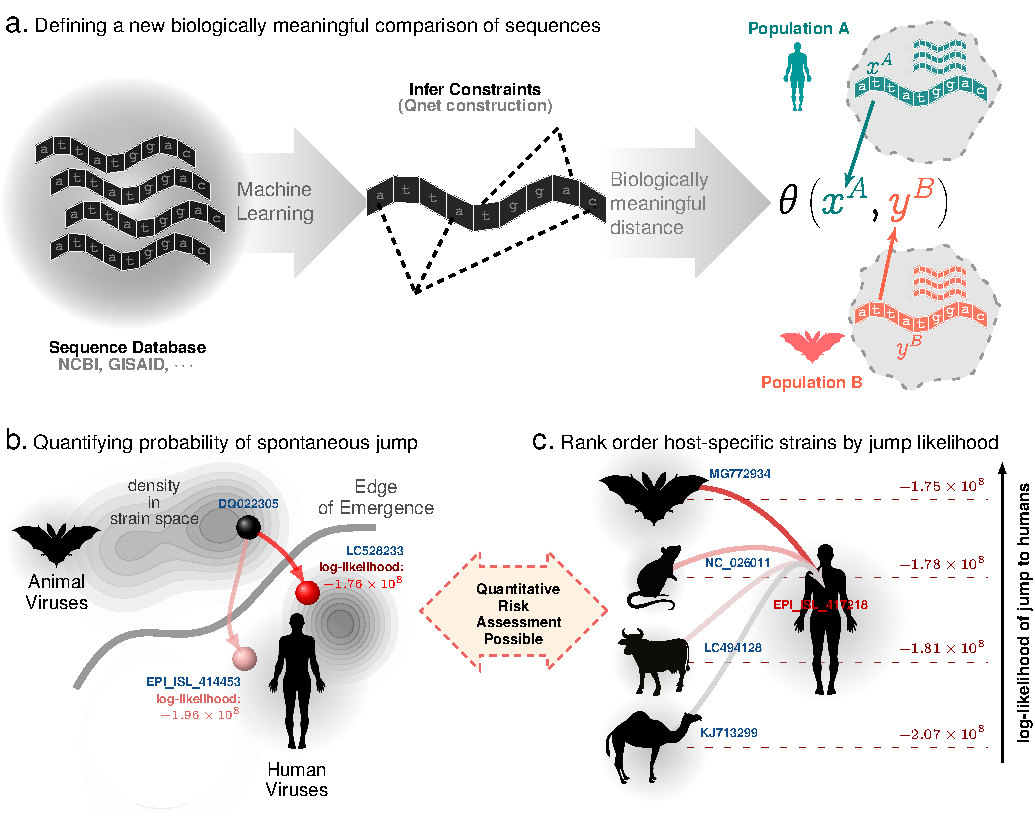
\includegraphics[width=0.95\textwidth]{Figures/External/tape.pdf}
  \fi
\vspace{-10pt}
 
\captionN{\textbf{Key insights: ability to quantify risk and rank-order strains.} \textbf{Panel a.} Using sequence variations observed in large databases, we distill evolutionary constraints on a genomic sequence to induce a biology-aware metric for comparing subtle differences in mutating sequences. This metric (q-distance) adjusts to specific organisms, background populations and selection pressures, and reflects the true likelihood of a spontaneous jump from one sequence to the other. We can use this sequence level metric to compute distances between a sequence and a population, and two populations.  \textbf{Panels b-c} illustrates that we can calculate bounds on the  exact likelihood of a spontaneous jump  between  strains (panel b) and rank-order strains observed in a diverse set of hosts to accurately model future emergence risk (panel c).}\label{figscheme}
\end{figure*}
\else
\refstepcounter{figure}\label{figscheme}
\fi
%#############################################
%#############################################

This is a major improvement over the existing state of art in phylogeny construction from sequences, which generally assume a model for character substitution (either for nucleotides or amino acid residues) ignoring the effect of selection and the existence of long-range complex dependencies in viable mutations along the genomic sequence. Notably, even relatively complex substitution models ($e.g.$ ones that allow site specific mutation rates) do not capture the effect of individual changes that may dramatically alter fitness in the environment. Our proposed approach, on the other hand, learns from and leverages these patterns, using sophisticated pattern discovery via novel machine learning algorithms. While the effect of the environment and selection cannot be inferred from a single sequence, an entire database of observed strains, processed through sophisticated learning, can parse out predictive models of these complex interactions. Our only intuitively well-justified assumption on the evolutionary dynamics is that more fit strains end up with more progenies (follows from definition of Malthusian fitness), and are thus more likely to be sampled in surveillance efforts (again, intuitively obvious).  Thus, in a strict mathematical sense, the distance we propose is not a distance between two strains $x,y$, but a distance between strain $x^A$ ($x$ in a background environment $A$) and a strain  $y^B$ ($y$ in a background environment $B$). Indeed we can show that the distance between the same pair of  strains of \infl HA is different based on if they are collected in 2008 vs in 2009, reflecting that the background environment and circulating diversity changed over the two years.  Thus, our  distance metric  is fundamentally different from measures that exist in the literature. In particular, our mathematical framework leads to the key result that the q-distance is a scaled representation of the log-likelihood of spontaneous jump  between strains. This interpretation is missing in existing tools, and makes way for leveraging the q-distance to model emergence of new strains. Thus, we can predict entirely new sequences -- which differ by a non-trivial number of edits from any observed strain -- that still lead to functional proteins, as demonstrated in our preliminary studies.

Very recently, two articles have explored the possibility of predicting  pathogenicity from genomic sequences (Mollentze~\cite{mollentze2021identifying}) and forecasting which amongst observed mutations will dominate the circulating population (Maher et al~\cite{maher2021predicting}). These studies provide strong pieces of evidence that challenge the idea that forecasting future variants of virus strains is impossible, while aligns with our goals. While their questions overlap with our framework, our approach is distinct and more ambitious. For example,  Mollentze  uses  classical  sequence similarity; extended to include similarity to  human housekeeping genes hoping to identify viruses  evading the human immune system more easily.  The demonstrated  performance is poor (incorrectly tagging all SARS-related coronaviruses as potentially pathogenic), implying un-actionable specificity. On the other hand,  Maher outright assumes mutations to be independent. Features are found manually,  are specific to \hcov, and the authors take  a meta-analysis-esque route, compiling together a ``kitchen-sink'' of features via standard machine learning. Importantly, these approaches  only aim to predict point mutations, with  the gargantuan complexity of tracking a more complete strain through a high-dimensional sequence space well beyond their conceptual limits. Thus, even the question if whether a yet-to-be-seen strain is indeed a valid biological encoding of a virus (which is simpler to determining risk posed by such future variants) cannot answered by our peers, limiting such approaches to analyzing mutations already seen, or strains  already collected.  Additionally, generalizability and actionability is  suspect, given that Maher's features are \hcov specific, and Mollentze's similarity to house-keeping genes might not be universal. Finally, both these  approaches apply to a mutation or a combination of mutations that already exist, and cannot predict new mutations, or new strains.





\section*{Methods}

Aiming to validate our metric in the context of  viral evolution, we begin by collecting over $98,000$ Influenza A HA/NA nucleotide sequences from two public databases (NCBI % \href{https://www.ncbi.nlm.nih.gov/genome/viruses/}{https://www.ncbi.nlm.nih.gov/genome/viruses/}
and GISAID; % \href{https://www.gisaid.org/}{https://www.gisaid.org/}
see SI-Table~\ref{SI-tabseq}), uncovering a network of  dependencies between individual mutations revealed through subtle variations of the aligned sequences. These dependencies define our organism-specific model referred to as the \textit{quasi-species network} or the \qnet (see Fig.~\ref{figscheme} and \ref{fig0}). The q-distance, informed by the dependencies modeled by the inferred {\qnet}s, adapts to the specific organism, allele frequencies, and variations in the background population. 

%#############################################
%#############################################
\ifFIGS
\begin{figure*}[!ht]
  \tikzexternalenable
  \tikzsetnextfilename{scheme}
  \centering 
  \iftikzX
  \input{Figures/fig0}  
  \vspace{0pt}   
  
  \else 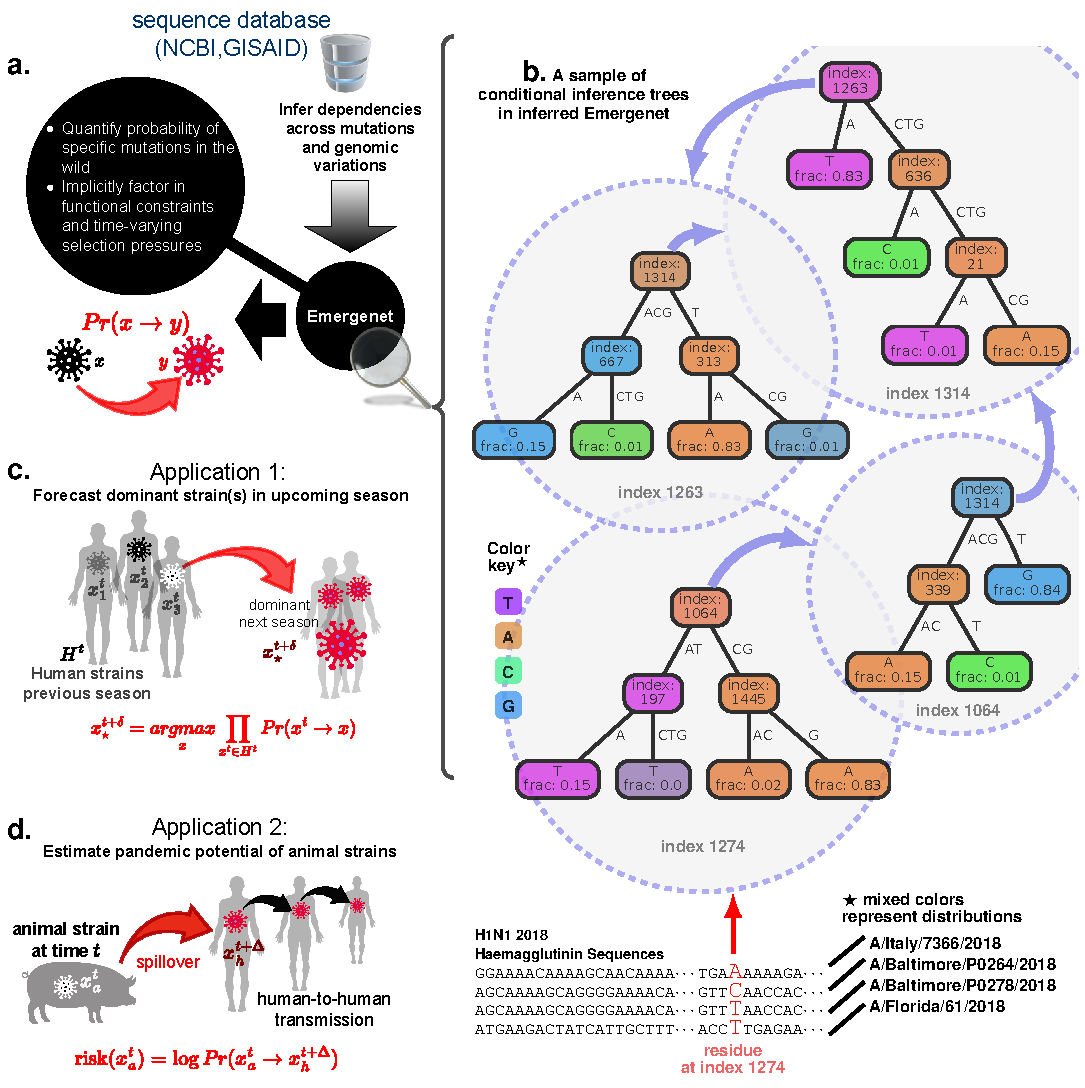
\includegraphics[width=0.97\textwidth]{Figures/External/scheme.pdf}
  \fi
  \captionN{\textbf{\qnet Computation scheme}. \textbf{Panel a}. 
As an example, beginning with aligned sequences, we calculate a conditional inference tree for index 1274, which involves indices 1064, 1445, 197 as predictive features. These features are automatically selected by the algorithm, as being maximally predictive of the base at 1274. Then, we compute predictors for each of these predictive indices, $e.g.$ we show the inference tree computed for index 1064, which involves index 1314 and 339 as features. Continuing, we find that the predictor for 1314 involves indices 1263, 636 and 21, and that for 1263 involves 1314, 667 and 313. Note that recursive dependencies arise automatically: the predictor for 1263  depends on 1314, and that for 1314 depends on 1263.  \textbf{Panels b-c} show \qnet dependency graphs for \hcov spike protein and Influenza A HA respectively, illustrating the distinct patterns of mutational constraints inferred. Both HA in Influenza A and the spike protein in \hcov are implicated in viral entry into host cells, and crucial for host specificity of infections. Additionally, the inferred structures underscore the significantly more complex dependencies in \hcov compared to Influenza A.}\label{fig0}
\end{figure*}
\else
\refstepcounter{figure}\label{fig0}
\fi
%#############################################
%#############################################

Using aligned genomic sequences sampled from  similar populations, $e.g.$ HA from Human Influenza A in year 2008, we construct the \qnet via  customized machine learning algorithms to  learn models for predicting the mutational variations at each sequence index using other indices  as features. For example, in Fig.~\ref{fig0}a,  the predictor for index 1274 uses variation at index 1064 as a feature, and the predictor for index 1064 uses index 1314 as a feature, and so on -- ultimately uncovering a recursive dependency structure. The \qnet predicts the nucleotide distribution over the base alphabet at any specific index, conditioned on the nucleotides making up the rest of the sequence of the gene or genome fragment under consideration. Aside from this example, amino acids sequences can also be used to train the \qnet. Finally, we define the q-distance (See Eq.~\eqref{q-distance} in Materials and Methods) as the square-root of the Jensen-Shannon (JS) divergence~\cite{cover} of these conditional distributions from one sequence to another, averaged over the entire sequence. Invoking Sanov's theorem on large deviations~\cite{cover}, we show  that the  likelihood of spontaneous change is bounded above and below by a simple exponential function of the  q-distance. 

The mathematical intuition behind relating the new distance to change-probability  is the same as in the prediction of  a biased outcome when we sequentially toss a fair coin. With an overwhelming probability, such an experiment with a fair coin should result in roughly equal number of heads and tails. However, ``large deviations'' can happen, and the probability of such rare events is quantifiable~\cite{varadhan2010large} with existing theory. We show here that the likelihood of a spontaneous transition of a genomic sequence to a  different variant by random chance may also be similarly bounded, given we have the \qnet as  an estimated model of the evolutionary constraints.

Importantly, the q-distance  between two sequences may change even if only the background population changes (See SI-Table~\ref{SI-tabex}, where  the distance between two  fixed sequences vary when we vary their collection years). Sequences may have a large q-distance and a small edit distance, and vice versa (although on average the two distances tend to be positively correlated, see SI-Table~\ref{SI-tabcor}).  Hence for tracking drift in Influenza A, we construct a seasonal \qnet for each sub-type and protein that we consider.

Our first application aims to predict dominant strains for the seasonal flu epidemic. Periodic adjustment of the Influenza vaccine components is necessary to account for antigenic drift~\cite{boni2008vaccination,dos2016influenza}. The flu shot in each hemisphere is annually prepared at least six months in advance, and is based on a cocktail of historical strains determined by the WHO via global surveillance~\cite{agor2018models}, hoping to match the circulating strain(s) in the upcoming flu season. A variety of hard-to-model effects hinder this prediction, which, despite observed cross-reactive effects~\cite{tricco2013comparing}, have limited vaccine effectiveness in recent years~\cite{cdceff}. For predicting future strains, we hypothesized that since the probability of a drift exponentially decreases with an increasing q-distance, the centroid of the strain distribution in our metric will change slowly. If true, the strain selected closest to the ``q''-centroid will be a good approximation of next season's dominant strain. We then computed the dominant strain in each season as the centroid of the strain distribution observed in a given season in the classical sense (no. of mutations), since the edit distance metric is widely used and offers a point of comparison between WHO predictions and \qnet predictions. Note that the recommendations for the northern hemisphere are given in February, while that for the southern hemisphere are given at the end of December the previous year, keeping in mind that the flu season in the south begins a few months early, as described in Fig.~\ref{figseasonal}. Finally, we computed the edit distance (no. of mutations) between the dominant strain and the WHO and \qnet predictions.

Our second application aims to compare emergence risk grades given by the CDC through its Influenza Risk Assessment Tool (IRAT) with results using our q-distance metric. While IRAT uses a combination of 10 weighted risk elements evaluated slowly over the course of several months per strain, we attempt to quantify emergence risk quickly with the q-distance metric. We looked at the same strains that were analyzed by IRAT. For each strain previously analyzed by IRAT, we construct \qnet models for HA and NA segments using all human strains of the same variety circulating in the year prior to risk assessment. For example, the "A/swine/Shandong/1207/2016" strain was assessed by IRAT in July 2020, so we will use human H1N1 strains circulating between July 1, 2019 through June 30, 2020. For sub-types with few human strains (H1N2, H5N1, H5N6, H7N7, H9N2), we only use the upper bound of the date. We then compute the average q-distance between the strain in question and the circulating human strains for both HA and HA segments. Seven of the 23 strains are not included in our comparison due to having zero or too few human strains in the sample space to construct a \qnet; see Supplementary Text, SI-Table~\ref{SI-irattab}. We hypothesize that a lower average q-distance between the strain in question and circulating human strains should correspond to a higher emergence risk. Hence, we expect to see a high negative correlation between q-distance and IRAT grade, which assigns 1 to be the lowest risk and 10 to be the highest risk.

 



\section*{Results} 

We tested the hypothesis of our first application, computing the strain closest to the ``q''-centroid for each flu season and selecting that strain as the prediction for the next season's dominant strain. We performed this analysis on past two decades of sequence data for Influenza A (H1N1 and H3N2) with promising results: the q-distance based prediction demonstrably outperforms WHO recommendations by reducing  the  distance between the predicted and  the dominant  strain (Fig.~\ref{figseasonal}). Recall that we identify the dominant strain to be the one that occurs most frequently, computed as the centroid of the strain distribution observed in a given season in the classical sense (no. of mutations).

%#############################################
%#############################################
\ifFIGS
\begin{table*}[!ht]\centering
\captionN{Out-performance of \qnet recommendations over WHO 
for Influenza A vaccine composition}\label{tabperf}\centering

\sffamily\fontsize{9}{9}\selectfont

\begin{tabular}{C{.5in}|C{.35in}|C{.7in}|C{0.35in}|C{0.35in}|C{0.4in}|C{0.35in}|C{0.35in}|C{0.4in}|C{0.35in}|C{0.35in}|C{0.4in}}
\multicolumn{3}{c}{}&\multicolumn{3}{c}{Two decades}&\multicolumn{3}{|c}{One decade}&\multicolumn{3}{|c}{2015-2019}\\\hline
Subtype & Gene & Hemisphere & WHO Error & \qnet Error & Improvement (\%) & WHO Error & \qnet Error & Improvement (\%) & WHO Error & \qnet Error &  Improvement (\%)\\\hline
H1N1&HA& North &12.67&8.76&30.83&4.38&1.19&72.83&2.52&0.33&86.79\\\hline
H1N1&HA& South &13.57&9.00&33.68&4.67&1.62&65.31&2.52&0.62&75.47\\\hline
\rowcolor{lightgray}H1N1&HA&Average&13.12&8.88&32.25&4.53&1.40&69.07&2.52&0.48&81.13\\\hline
H3N2&HA& North &7.65&4.71&38.46&5.00&2.94&41.18&1.82&0.88&51.61\\\hline
H3N2&HA& South &7.59&4.82&36.43&4.94&3.00&39.29&1.82&0.94&48.39\\\hline
\rowcolor{lightgray}H3N2&HA&Average&7.62&4.77&37.44&4.97&2.97&40.24&1.82&0.91&50.00\\\hline
H1N1&NA& North &8.29&6.90&16.67&2.62&1.10&58.18&2.10&0.48&77.27\\\hline
H1N1&NA& South &9.14&8.38&8.33&3.00&1.43&52.38&2.10&0.76&63.64\\\hline
\rowcolor{lightgray}H1N1&NA&Average&8.72&7.64&12.50&2.81&1.27&55.28&2.10&0.62&70.46\\\hline
H3N2&NA& North &4.21&3.63&13.75&2.11&1.79&15.00&1.32&0.32&76.00\\\hline
H3N2&NA& South &4.68&4.16&11.24&2.58&2.05&20.41&1.32&0.42&68.00\\\hline
\rowcolor{lightgray}H3N2&NA&Average&4.44&3.90&12.50&2.34&1.92&17.70&1.32&0.37&72.00\\\hline
\end{tabular}

\end{table*}
\else
\refstepcounter{table}\label{tabperf}
\fi
%#############################################
%#############################################

The \qnet single-cluster predictions consistently outperform the WHO recommendations. For H1N1 HA, the \qnet induced recommendation outperforms the WHO suggestion by $>33\%$ on average over the last two decades, and $>71\%$ on average in the last decade. The gains for H1N1 NA over the same time periods are $>15\%$ and $>52\%$, respectively. For H3N2 HA, the \qnet induced recommendation outperforms the WHO suggestion by $>37\%$ on average over the last two decades, and $>40\%$ in the last decade. The gains for H3N2 NA over the same time periods are $>14\%$ and $>15\%$, respectively. Finding multi-cluster predictions has the potential to yield even more improved results, as seen in Fig.~\ref{figseasonal} and SI-Table~\ref{SI-tabrec8} through SI-Table~\ref{SI-tabrec11}.

The full table of single-cluster results with improvement broken down by hemisphere is given in Table~\ref{tabperf}. Fig.~\ref{figseasonal} illustrates the relative gains computed for both subtypes and the two hemispheres (since the flu season occupy distinct time periods and may have different dominant strains in the northern and southern hemispheres~\cite{boni2008vaccination}). Additional improvement is possible if we recommend multiple strains every season for the vaccine cocktail (Fig.~\ref{figseasonal}e,f,k,l). The details of the specific strain  recommendations made by the \qnet approach for two subtypes (H1N1, H3N2), for two genes (HA, NA) and for the northern and the southern hemispheres over the previous two decades are enumerated in the Supplementary Text in Tables SI-Table~\ref{SI-tabrec0} through SI-Table~\ref{SI-tabrec11}.

We hypothesized in our second application that there will be a high negative correlation between q-distance and IRAT emergence grade. Plotting our results in Fig.~\ref{figirat}, we find a correlation of $-0.7032$ $(p < 0.005)$, which is statistically and substantively significant. We can conclude, therefore, that a lower averae q-distance to currently circulating human strains corresponds to a higher risk of emergence with respect to the CDC's grades. Due to the small number of Influenza A strains that have been analyzed by IRAT, we should be wary of the realistic statistical significance of our results. Achieving a moderately high correlation coefficient and p-value is nevertheless a positive result, and further uncovers the potential of our model to quantify risk of emergence. 

For further analysis, we also performed q-analysis on IRAT H1- and H3- sub-types by taking average q-distance between the target strain and all human-circulating strains available, with no upper or lower collection date bound. We expected the correlation to be worse than with bounded strains, since a strain being ``close" to humans at some point in the past does not necessarily mean being close now. Indeed, our results showed almost no correlation to the IRAT emergence risk scores. Bounded results for H1- and H3- sub-types yielded a correlation of $-0.6916$, while unbounded results yielded a correlation of $0.0545$; see SI-Fig.~\ref{SI-irat}.

Given the efficiency of the q-distance computations, we can track how risk of emergence changes over time by continually updating the current human-circulating strains each year. For exact average q-distance and \qnet sample size statistics, please see SI-Table~\ref{SI-irattab} in the Supplementary Text.

%#############################################
%#############################################
\ifFIGS
\begin{figure*}[!ht]
  \tikzexternalenable
  \tikzsetnextfilename{scheme}
  \centering 
  \iftikzX
  \input{Figures/External/irat_combined.png}  
  \vspace{0pt}   
  
  \else 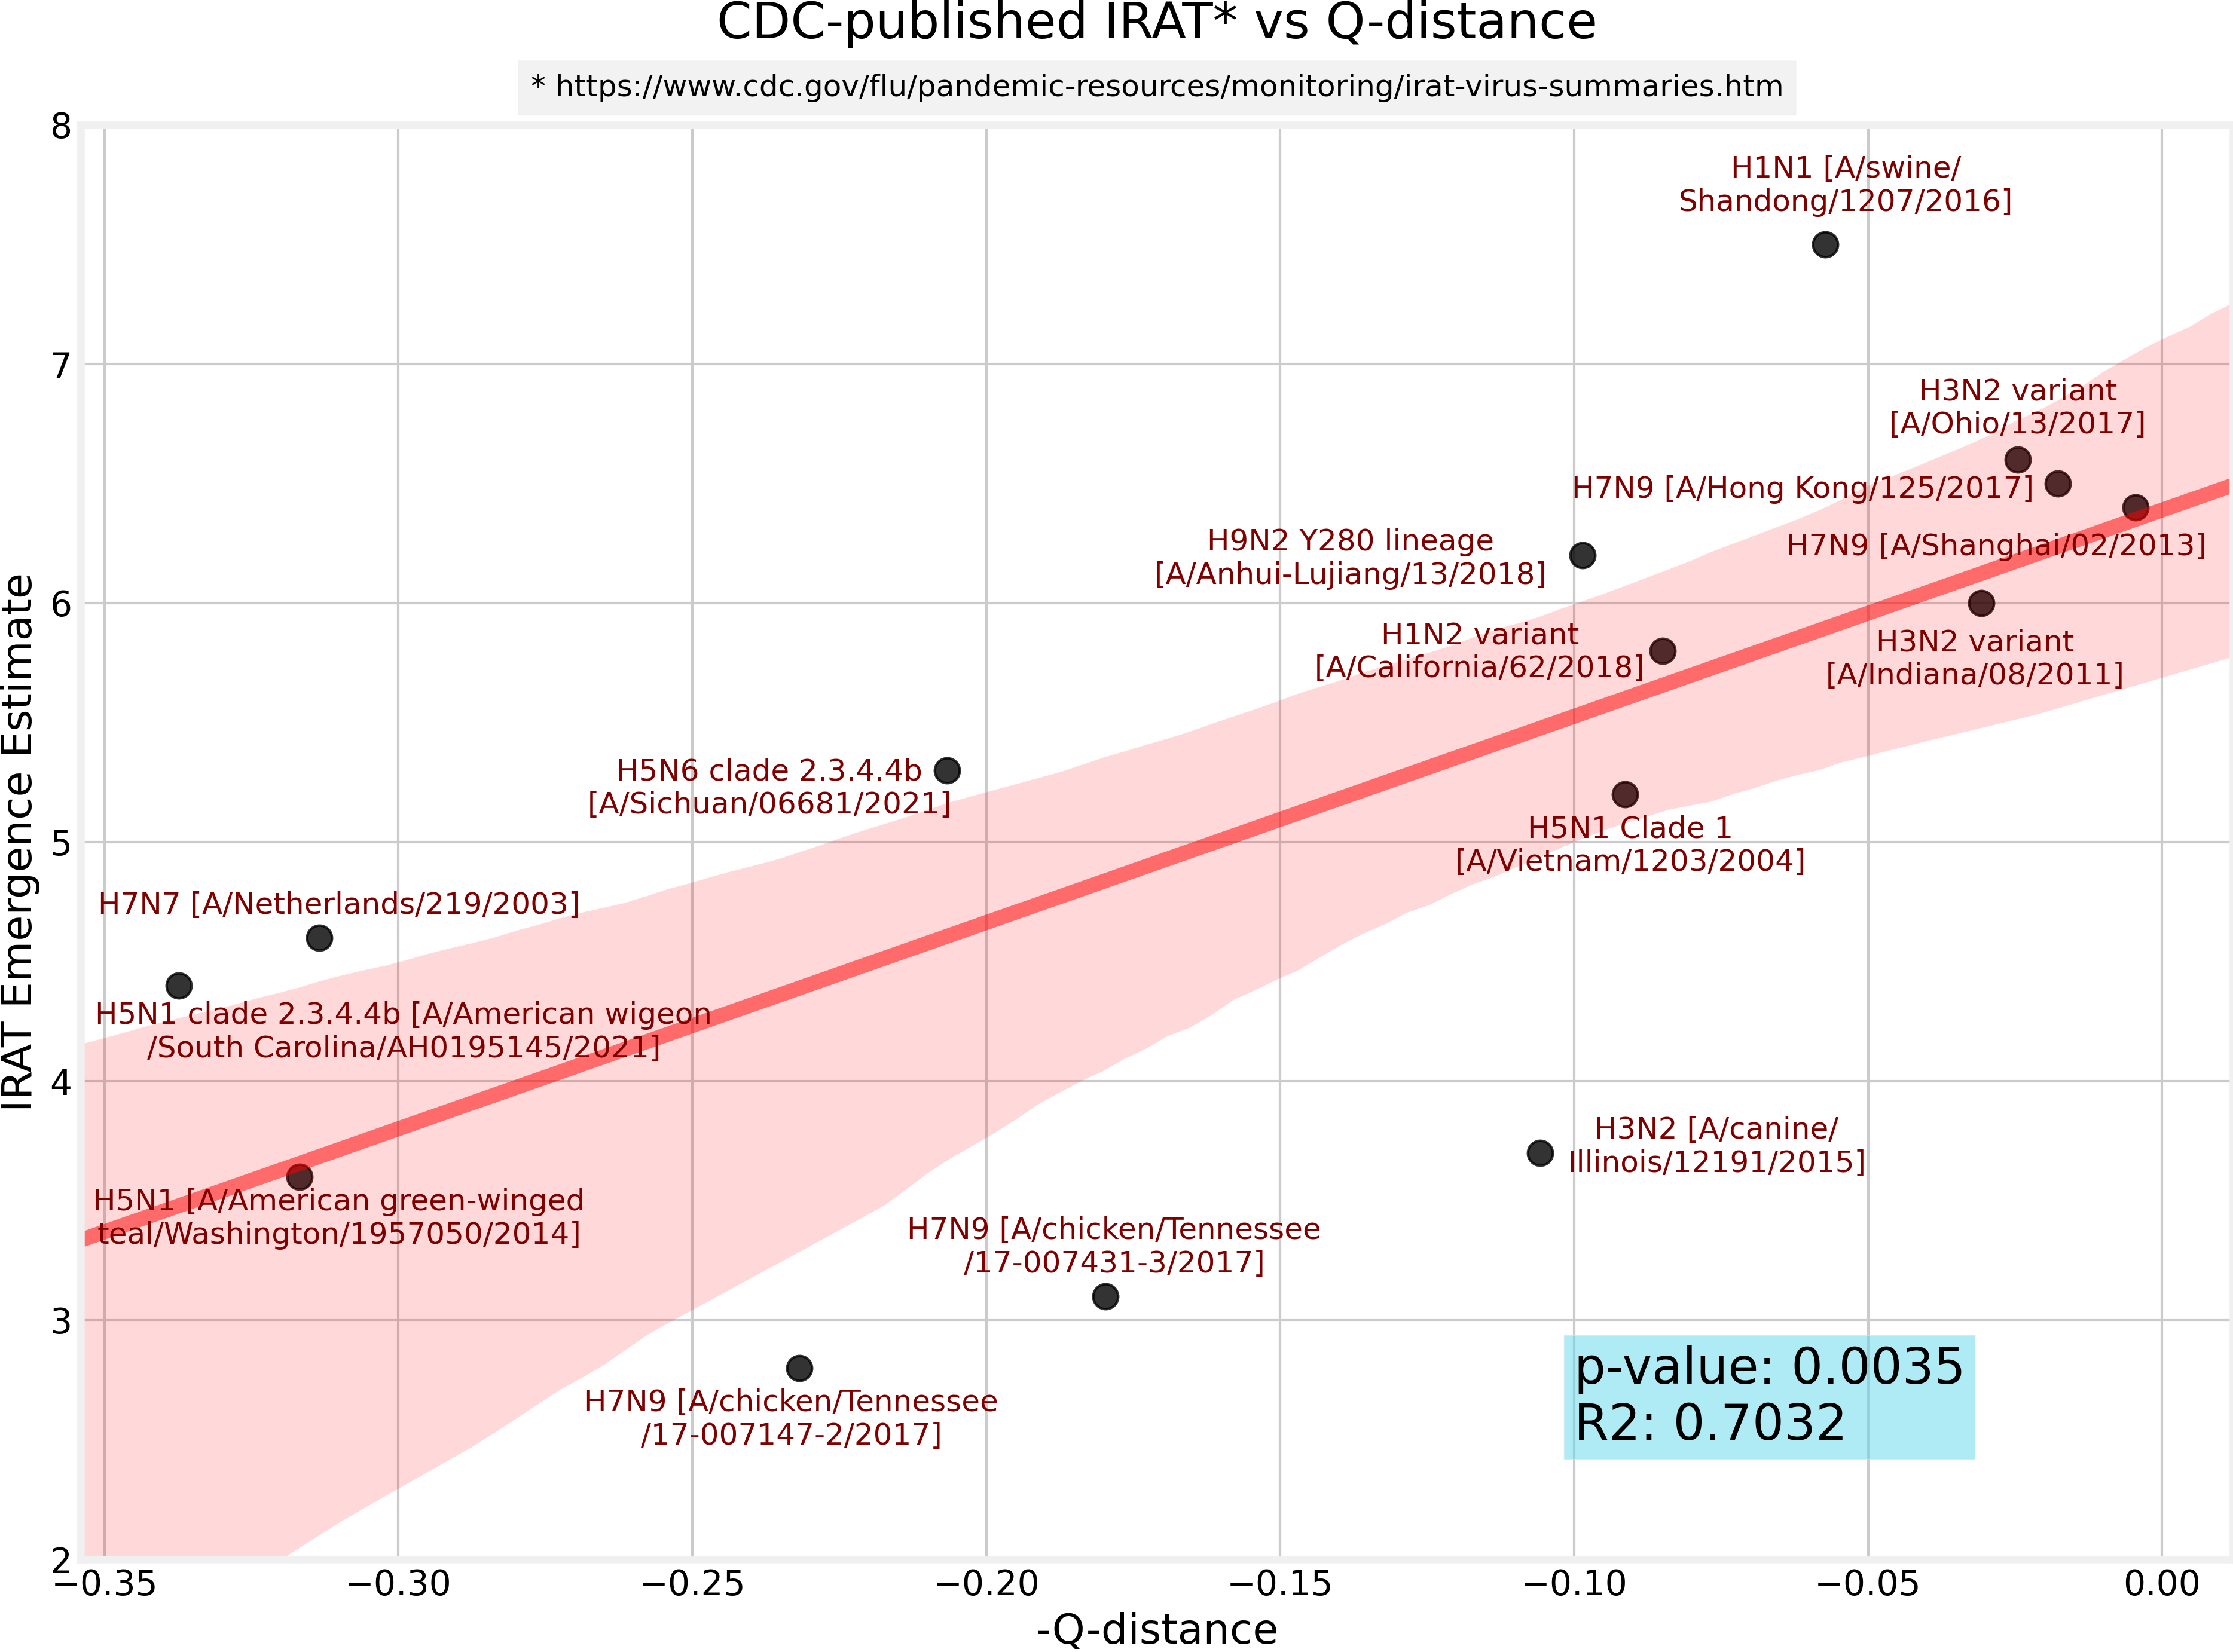
\includegraphics[width=0.9\textwidth]{Figures/External/IRAT_combined.png}
  \fi
  \captionN{\textbf{IRAT emergence risk vs. q-distance}. There is an approximate linear relationship between average q-distance from human circulating strains (averaged across both HA and NA) and IRAT emergence risk grade. Note that IRAT has released results for 23 strains to date, but only 15 are plotted on the graph. This is because the strains not pictured have less than 30 human strains of the same sub-type, so a sufficiently representative \qnet could not be trained.
  }\label{figirat}
\end{figure*}
\else
\refstepcounter{figure}\label{figirat}
\fi
%#############################################
%#############################################





\section*{Discussion \& Sequence Comparisons}

For further discussion, we looked at our \qnet predictions more closely. Comparing the \qnet inferred strain (QNT) against the one recommended by the WHO, we find: 1) the residues that only the QNT matches correctly with DOM (while the WHO fails) are largely localized within the receptor binding domain (RBD), with $>57\%$ occurring within  the RBD on average (see Fig.~\ref{figseq}a for a specific example), and 2) when the WHO strain deviates from  the QNT/DOM  matched residue, the ``correct'' residue is often replaced in the WHO recommendation with one that has very different side chain, hydropathy  and/or chemical properties (See Fig.~\ref{figseq}b-f), suggesting deviations in recognition characteristics. Combined with the fact that we find circulating strains are almost always within a few edits of the DOM (See SI-Fig.~\ref{SI-figdom}), these observations suggest that hosts vaccinated with the QNT recommendation is more likely to have season-specific antibodies that are more likely to recognize a larger cross-section of the circulating strains.

High season-to-season genomic variation in the key  Influenza capsidic proteins is driven by two opposing influences: 1) the need to conserve function  limiting random mutations, and 2) hyper-variability to escape recognition by neutralizing antibodies. Even a  single residue change in the surface proteins might dramatically alter recognition characteristics, brought about by unpredictable~\cite{carugo2001normalized,righetto2014comparative} changes in local or regional properties such as charge, hydropathy, side chain solvent accessibility~\cite{lee1971interpretation,shrake1973environment,momen2008impact,adamczak2005combining}.

Focusing on the average localization of the QNT to WHO deviations in the HA molecular  structure, the changes are observed to primarily occur in the HA1 sub-unit (See Fig.~\ref{figseq}g-i, HA0 numbering used, other numbering conversions are given in SI-Table~\ref{SI-tabnum}), with the most frequent deviations  occurring around the $\approx 200$ loop, the $\approx 220$ loop, the $\approx 180$ helix, and the $\approx 100$ helix, in addition to some residues in the HA2 sub-unit ($\approx 49$ \& $\approx 124$). Unsurprisingly, the residues we find to be most impacted in the HA1 sub-unit (the globular top of the fusion protein) have been repeatedly implicated in receptor binding interactions~\cite{tzarum2015structure,lazniewski2018structural,garcia2015dynamic}. Thus, we are able to fine tune the future recommendation over the state of the art, largely by modifying residue recommendations around the RBD and  structures affecting recognition dynamics.





\section*{Limitations \& Conclusion}

Calculation of q-distance  is currently limited to similar and aligned sequences, $e.g.$  Influenza strains from different sub-types, hosts or seasons. Furthermore, we need a sufficient diversity of observed strains to successfully construct the \qnet. A multi-variate regression analysis indicates  that the most important factor for our approach to succeed is  the diversity of the sequence dataset (see Supplementary Text, SI Table~\ref{SI-tabreg}). Arguably, simply reducing the edit distance from the dominant strain is not guaranteed to translate to a better immunological protection. Nevertheless, consistent improvement in this metric achieved purely via computational means suggests the possibility of improvement over current practice. 

In conclusion, we introduce a data-driven distance metric to track subtle deviations in sequences. We show that we can use the q-distance metric to make recommendations for the flu-shot composition, outperforming the WHO's recommendations in relation to the dominant strain. We also show that we can roughly replicate the CDC's IRAT grades for emergence risk of strains not currently circulating among humans in an efficient manner that can be scaled to rank many more strains than is currently done. The ability to predict future flu strains via subtle variations in a limited set of immunologically important residues suggest that the tools developed here could lead to more effective escape-resistant vaccines, which could be essential in preempting and mitigating the next pandemic.





\allowdisplaybreaks{
We briefly describe the proposed computational framework. 


\subsection*{\enet Framework}
We do not assume that the mutational  variations at the individual indices of a genomic sequence are independent (See Fig~\ref{figscheme}a). Irrespective of whether mutations are truly random~\cite{hernandez2018algorithmically}, since only certain combinations of individual mutations are viable, individual mutations across a genomic sequence replicating in the wild  appear  constrained, which is what is explicitly  modeled in our approach.

% 

Consider a set of random variables $X=\{X_i\}$, with $i \in \{1, \cdots, N\}$, each taking value from the respective sets $\Sigma_i$. Here each $X_i$ is the random variable modeling the ``outcome'' $i.e.$ the AA residue at the $i^{th}$ index of the protein sequence. A sample $x \in \prod_1^N \Sigma_i$ is an ordered $N$-tuple, which is a specific strain in this context,  consisting of a realization of each of the variables $X_i$ with the $i^{th}$ entry $x_i$ being the realization of random variable $X_i$.

We use the notation $x_{-i}$ and $x^{i,\sigma}$ to denote:
\begin{subequations}\cgather{
x_{-i} \triangleq x_1, \cdots, x_{i-1},x_{i+1},\cdots,x_N\\
x^{i,\sigma} \triangleq x_1, \cdots, x_{i-1},\sigma,x_{i+1},\cdots,x_N, \sigma \in \Sigma_i
}\end{subequations} Also, $\Dx(S)$ denotes the set of probability measures on  a set $S$, $e.g.$,  $\D$ is the set of  distributions on  $\Sigma_i$.

We note that $X$ defines a random field~\cite{vanmarcke2010random} over the index set $\{1, \cdots, N\}$. 

\begin{defn}[\enet]
For a random field $X=\{X_i\}$ indexed by $i \in \{1, \cdots, N\}$, the \enet is defined to be the set of predictors $\Phi=\{\qn\}$, $i.e.$, we have:
\cgather{
\qn : \prod_{j \neq i} \Sigma_j \rightarrow \D,
}  where for a sequence $x$, $\Phi_i(x_{-i}) $ estimates the distribution of $X_i$ on the set $\Sigma_i$.
\end{defn}
We use conditional inference trees as models for predictors~\cite{Hothorn06unbiasedrecursive}, although more general models are possible.





\subsection*{Biology-Aware Distance Between Sequences}
The mathematical form of our metric is not arbitrary; JS divergence is a symmetricised version of the more common KL divergence~\cite{cover} between distributions, and among  different possibilities, the \qdist  is the simplest metric such that the likelihood of a spontaneous jump (See Eq.~\eqref{fundeq} in Methods) is provably bounded above and below  by simple exponential functions of the \qdist.

\begin{defn}[\qdist: adaptive biologically meaningful dissimilarity between sequences]\label{defqdistance}
Given two sequences $x,y \in \prod_1^N\Sigma_i$, such that $x,y$ are drawn from the  populations $P,Q$  inducing the \enet $\Phi^P,\Phi^Q$, respectively,  we define a pseudo-metric $\theta(x,y) $, as follows:
\cgather{\label{q-distance}
\theta(x,y) \triangleq \mathbf{E}_i \left (  \J^{\frac{1}{2}} \left (\qn^P(x_{-i}) , \qn^Q(y_{-i})\right ) \right )
} 
where $ \J(\cdot,\cdot)$ is the Jensen-Shannon divergence~\cite{manning1999foundations} and $\mathbf{E}_i$ indicates expectation over the indices.
\end{defn}
The square-root in the definition arises naturally from the bounds we are able to prove, and is dictated by the form of Pinsker's inequality~\cite{cover}, ensuring that   the sum of the length of successive path fragments equates the length of the path.%, making it possible to use standard  algorithms  for q-phylogeny construction.


%\subsection*{Significance Test for Population Membership}
\subsection*{Membership Degree}

For our modeling to be reliable, we need a quantitative test of how well the \enet represents the data. Here, we formulate an explicit membership test to ascertain if individual samples may indeed be generated by the \enet with sufficiently high probability.
%
\begin{defn}[Membership probability of a sequence]\label{defmem}
Given a population $P$ inducing the \enet $\Phi^P$ and a sequence $x$, we can compute the membership probability of $x$:
\cgather{
\mem{x}^P \triangleq Pr(x \in P) = \prod_{j=1}^N \left ( \Phi^P_j(x_{-j}) \vert_{x_j} \right )
}
\end{defn}
$x_j$ is the $j^{th}$ entry in $x$, and is thus an element in the set $\Sigma_j$. Since we are mostly concerned with the case where $\Sigma_j$ is a finite set, $\Phi^P_j(x_{-j}) \vert_{x_j}$ is the entry in the probability mass function corresponding to the element of $\Sigma_j$ which appears at the  $j^{th}$ index in sequence $x$. 
 
We can carry out this calculation for a sequence $x$  known to be in the population $P$ as well, which allows us to define the membership degree $\M^P_x$.
\begin{defn}[Membership degree]
Let $X$ be a random field representing a population $P$, $ie.$. $X=x$ is a randomly drawn sequence from $P$. Then  the membership degree $\M^P$ is  a function of the random variable $X$: 
\cgather{
\M^P(X)  \triangleq  \prod_{j=1}^N \left ( \Phi^P_j(X_{-j}) \vert_{X_j} \right )
}Note that $\M^P$ takes values in the unit interval $[0,1]$, and the probability  $x$ is a member of the population $P$ is $\M^P(X=x)$, denoted briefly as $\mem{x}^P$ or $\mem{x}$ if $P$ is clear from context.
\end{defn}
Since $\M^P(X)$ is a random variable, we can now compute sets of sequences that better represent the population $P$, and ones that are on the fringe. We can also evaluate using a pre-specified significance-level if a particular sequence is not from the population $P$.



\subsection*{Theoretical Probability Bounds}

The \enet framework  allows us to rigorously compute bounds on the probability of a spontaneous change of one strain to another, brought about by chance mutations. While any sequence of mutations is equally likely, the ``fitness'' of the resultant strain, or the probability that it will even result in a viable strain, or not. Thus the necessity of preserving  function  dictates that not all random changes  are viable, and the probability of observing some trajectories through the sequence space  are far greater  than others. The \enet framework allows us to explore this constrained dynamics, as revealed by a sufficiently large set of genomic sequences.



The mathematical intuition  relating  \qdist  to the log-likelihood of spontaneous change  is similar to quantifying the  odds of  a rare biased outcome when we  toss a fair coin.
While for an unbiased coin, the odds of roughly 50\% heads is overwhelmingly likely, large deviations do happen rarely, and it turns out that the probability of such rare deviations can be explicitly quantified with existing statistical theory~\cite{varadhan2010large}.
 Generalizing to non-uniform conditional distributions inferred by the \enet, the likelihood of a spontaneous transition  by random chance may also be similarly bounded.


We show in Theorem~\ref{thmbnd} in the supplementary text that at a significance level $\alpha$, with a sequence length $N$, the probability of spontaneous jump of sequence $x$ from population $P$ to sequence $y$ in population $Q$, $Pr(x \rightarrow y)$, is bounded by:
\cgather{\label{fundeq}
\mem{y}^Q e^{ \frac{\sqrt{8}N^2}{1-\alpha}\theta(x,y)} \geqq Pr(x \rightarrow y) \geqq \mem{y}^Q e^{-\frac{\sqrt{8}N^2}{1-\alpha}\theta(x,y)}}
where $\mem{y}^Q$ is the membership probability of strain $y$ in the target population, $N$ is the sequence length, and $\alpha$ is the statistical signifacnce level.


\subsection*{Predicting Dominant Seasonal Strains} 

Analyzing the distribution of sequences observed to circulate in the human population at the present time allows us to forecast dominant strain(s) in the next flu season as follows:

Let $\dst$ be a dominant strain in the upcoming flu season at time $t+\delta$,
where $H^t$ is the set of observed strains presently in circulation in the human population (at time $t$). We will assume that the \enet is constructed using the sequences in teh set $H^t$, and remains unchanged upto $t+\delta$. Since this set is a function of time, the inferred \enet also changes with time, and the induced \qdist is denoted as $\theta^{[t]}(\cdot,\cdot)$.

From the RHS bound established in Theorem~\ref{thmbnd} (See Eq.~\eqref{fundeq} above) in the supplementary text, we have:
%
\calign{
  &\ln  \frac{Pr(x \rightarrow \dsta)}{\mem{\dsta}} \geqq  -\frac{\sqrt{8}N^2}{1-\alpha}\theta^{[t]}(x,\dsta)\\
\Rightarrow &\sum_{x \in H^t} \ln  \frac{Pr(x \rightarrow \dsta)}{\mem{\dsta}}  
\geqq  \sum_{x \in H^t}-\frac{\sqrt{8}N^2}{1-\alpha}\theta^{[t]}(x,\dsta)\\
\Rightarrow  &\sum_{x\in H^t}  \theta^{[t]}(x,\dsta) - \abs{H^t}A \ln \mem{\dsta} \geqq  A \ln \frac{1}{\prod_{x \in H^t} Pr(x \rightarrow \dsta)} \intertext{where $A =\frac{1-\alpha}{\sqrt{8}N^2} $, where $N$ is the sequence length considered, and $\alpha$ is a fixed significance level. Since minimizing the LHS maximizes the lower bound on the probability of the observed strains simultaneously giving rise to $\dsta$, a dominant strain  $\dst$ may be estimated as a solution to the optimization problem:}
&\dst = \argmin_{y \in \cup_{\tau \leqq t} H^\tau} \sum_{x\in H^t}  \theta^{[t]}(x,y) - \abs{H^t}A \ln \mem{y}
}%
%
\subsection*{Measure of Pandemic Potential}
\def\ast{x_a^t}
\def\hst{x_h^{t+\delta}}

We measure the potential of an animal strain $\ast$ to spillover and become HH capable as a human strain $\hst$, via the proposed \erisk defined as follows:
\cgather{\label{erisk}
\rho(\ast) \triangleq -\frac{1}{\abs{H^t}} \sum_{x \in H^t} \theta^{[t]}(\ast,x)
}%
where as before $H^t$ is the set of human strains observed recently (we take this as strains collected within the past year), and $\theta^{[t]}$ is the \qdist induced by the \enet computed from the sequences in $H^t$.

The intuition here is that a lower bound of $\rho(\ast)$ scales as average log-likelihood of the $\ast$ giving rise to a human strains in circulation at time $t$. Since the strains in $H^t$ are already HH capable, a high average likelihood of producing a similar strain has a high potential of being a HH cabale novel variant, which is a necessary condition of a pandemic strain. To establish the lower bound, we note that from  Theorem~\ref{thmbnd} (See Eq.~\eqref{fundeq} above) in the supplementary text, we have:
%
\cgather{
  \sum_{y \in H^t}\ln \abs{\frac{Pr(\ast \rightarrow y)}{\mem{y}}} \leqq -\frac{\sqrt{8}N^2}{1-\alpha} \abs{H^t}  \rho(\ast) \intertext{Denoting, $A =\frac{1-\alpha}{\sqrt{8}N^2} $,  $A\ln(\prod_{y \in H^t}\mem{y}) = C$, and $\langle \cdot \rangle$ as the geometric mean function, we have:}
\Rightarrow  \rho(\ast) \geqq A \ln \left (\prod_{y \in H^t}Pr(\ast \rightarrow y)\right )^{1/\abs{H^t}} + C \\
\Rightarrow \rho(\ast) \geqq A \ln \left \langle Pr(\ast \rightarrow \hst) \right \rangle + C
}%
Noting that $A,C$ are not functions of $\ast$, we conclude that a lower bound of the proposed risk measure $\rho(\cdot)$ scales with the average loglikelihood  of producing strains close to a circulating human strain at the current time. 

\subsection*{Proof of Probability Bounds}\label{sec:proof}

\begin{thm}[Probability bound]\label{thmbnd}
Given a sequence  $x$ of length $N$ that transitions  to a strain $y\in Q$, we have the following bounds at significance level $\alpha$.
\cgather{
\mem{y}^Q e^{ \frac{\sqrt{8}N^2}{1-\alpha}\theta(x,y)} \geqq Pr(x \rightarrow y) \geqq \mem{y}^Q e^{-\frac{\sqrt{8}N^2}{1-\alpha}\theta(x,y)}
  }%
  where $\mem{y}^Q$ is the membership probability of strain $y$ in the target population $Q$ (See Def.~\ref{defmem}), and $\theta(x,y)$ is the q-distance between $x,y$ (See Def.~\ref{defqdistance}).
\end{thm}
\begin{proof}
Using Sanov's theorem~\cite{cover} on large deviations, we conclude that the probability of spontaneous jump from strain $x\in P$ to strain $y\in Q$, with the possibility $P \neq Q$, is given by:
\cgather{\label{eq29}
  Pr(x\rightarrow y) =\prod_{i=1}^N \left ( \Phi^P_i(x_{-i}) \vert_{y_i} \right )
}
Writing the factors on the right hand side as:
\cgather{
 \Phi^P_i(x_{-i}) \vert_{y_i} =  \Phi^Q_i(y_{-i}) \vert_{y_i} \left (  \frac{\Phi^P_i(x_{-i}) \vert_{y_i}}{\Phi^Q_i(y_{-i}) \vert_{y_i}}  \right )
}%
we note that $\Phi^P_i(x_{-i})$, $\Phi^Q_i(y_{-i})$ are distributions on the same index $i$, and hence:
  \cgather{
\vert  \Phi^P_i(x_{-i})_{y_i} - \Phi^Q_i(y_{-i})_{y_i}\vert \leqq \sum_{y_i \in \Sigma_i} \vert  \Phi^P_i(x_{-i})_{y_i} - \Phi^Q_i(y_{-i})_{y_i}\vert 
}%
Using a standard refinement of Pinsker's inequality~\cite{fedotov2003refinements}, and the relationship of Jensen-Shannon divergence with  total variation, we get:
\cgather{
  \theta_i \geqq \frac{1}{8} \vert  \Phi^P_i(x_{-i})_{y_i} - \Phi^Q_i(y_{-i})_{y_i}\vert^2
\Rightarrow \left   \lvert  1  - \frac{\Phi^Q_i(y_{-i})_{y_i}}{\Phi^P_i(x_{-i})_{y_i}} \right \rvert \leqq \frac{1}{a_0}\sqrt{8 \theta_i}
}%
where $a_0$ is the smallest non-zero probability value of generating the entry at any index. We will see that this parameter is related to statistical significance of our bounds. First, we can formulate a lower bound as follows:
\cgather{\label{eqLB}
 \log \left  ( \prod_{i=1}^N   \frac{\Phi^P_i(x_{-i}) \vert_{y_i}}{\Phi^Q_i(y_{-i}) \vert_{y_i}}  \right )
  = \sum_i \log  \left  (  \frac{\Phi^P_i(x_{-i}) \vert_{y_i}}{\Phi^Q_i(y_{-i}) \vert_{y_i}}  \right )
\geqq \sum_i \left  ( 1- \frac{\Phi^Q_i(y_{-i})_{y_i}}{\Phi^P_i(x_{-i})_{y_i}} \right ) \geqq  \frac{\sqrt{8}}{a_0}\sum_i\theta_i^{1/2} = -\frac{\sqrt{8}N}{a_0}\theta
}%
Similarly,  the upper bound may be derived as:
\cgather{\label{eqUB}
\log \left  ( \prod_{i=1}^N   \frac{\Phi^P_i(x_{-i}) \vert_{y_i}}{\Phi^Q_i(y_{-i}) \vert_{y_i}}  \right )
  = \sum_i \log  \left  (  \frac{\Phi^P_i(x_{-i}) \vert_{y_i}}{\Phi^Q_i(y_{-i}) \vert_{y_i}}  \right ) \leqq \sum_i \left  ( \frac{\Phi^Q_i(y_{-i})_{y_i}}{\Phi^P_i(x_{-i})_{y_i}} - 1 \right ) \leqq \frac{\sqrt{8}N}{a_0}\theta
}%
Combining Eqs.~\ref{eqLB} and \ref{eqUB}, we conclude:
\cgather{
\mem{y}^Q e^{ \frac{\sqrt{8}N}{a_0}\theta} \geqq Pr(x \rightarrow y) \geqq \mem{y}^Q e^{-\frac{\sqrt{8}N}{a_0}\theta}
}%
Now, interpreting $a_0$ as the probability of generating an unlikely event below our desired threshold ($i.e.$ a ``failure''), we note that the probability of generating at least one such event is given by $1-(1-a_0)^N$. Hence if $\alpha$ is the pre-specified significance level, we have for $N >> 1 $:
\cgather{
 a_0 \approx (1 -\alpha)/N
}%
Hence, we conclude, that at significance level $\geqq \alpha$, we have the bounds:
\cgather{
\mem{y}^Q e^{ \frac{\sqrt{8}N^2}{1-\alpha}\theta} \geqq Pr(x \rightarrow y) \geqq \mem{y}^Q e^{-\frac{\sqrt{8}N^2}{1-\alpha}\theta}
  }%
\end{proof}
\begin{rem}
This bound can be rewritten in terms of the log-likelihood of the spontaneous jump and  constants independent of the  initial sequence $x$ as:
\cgather{
\left \lvert \log Pr(x \rightarrow y) -C_0 \right \vert \leqq C_1 \theta
}%
where the constants are given by:
\calign{
C_0 &= \log \mem{y}^Q \\
C_1 &= \frac{\sqrt{8} N^2}{1-\alpha}
}%
\end{rem}


\subsection*{In-silico Corroboration of \enet{'s} Capability To Capture Biologically Meaningful Structure}
We compare the results of simulated mutational perturbations to sequences from our databases (for which we have already constructed \enet{s}), and then use NCBI BLAST (\href{https://blast.ncbi.nlm.nih.gov/Blast.cgi}{https://blast.ncbi.nlm.nih.gov/Blast.cgi}) to identify  if  our perturbed sequences match with existing sequences in the databases (\SUPPLEMENTARY Fig.~S-\ref{figsoa}). We find that in contrast to random variations, which rapidly diverge the trajectories, the \enet constraints tend to produce smaller variance in the trajectories, maintain a high degree of match as we extend our trajectories, and produces matches closer in time to the collection time of the  initial sequence, suggesting that the \enet  does indeed capture realistic constraints.


\subsection*{Multivariate Regression to Understand Data Characteristics Necessary For \enet Modeling}

We investigate the key factors that contribute to modeling a set of strains well within the \enet framework. We carry out a multivariate regression with data diversity, the complexity of inferred \enet and the edit distance of the WHO recommendation from the dominant strain as independent variables (See \SUPPLEMENTARY Table~S-\ref{tabreg} for definitions). Here we define data diversity as the number of clusters we have in the input set of sequences, such that any two sequences five or less mutations apart are in the same cluster. \enet complexity is measured by the number of decision nodes in the component decision trees of the recursive forest.

We select several plausible structures of the regression equation, and in each case conclude that  data diversity has the most important and statistically significant contribution (\SUPPLEMENTARY Table~S-\ref{tabreg}).

\subsection*{Multivariate Regression to Identify Map from \qdist to Estimated IRAT scores}
We train separate General Linear Models (GLM) to estimate IRAT scores (emergence and impact) with average \qdist of a sequence of interest from a set of human strains, considering HA and NA sequences separately, using the CDC computed IRAT scores as the dependent variables. We also  include the geometric mean of the HA and NA based \qdist{s} as a potential explanatory variables. We use a standard Gaussian model family with identity link function to keep our model that maps \qdist{s}  to the IRAT scores as simple as possible (see \SUPPLEMENTARY Table~S-\ref{tabregGLMemergence}).


 



}





\section*{Data Sharing} 

Working software is publicly available at \href{https://pypi.org/project/quasinet/}{https://pypi.org/project/quasinet/}.
Accession numbers of all sequences used, and acknowledgement documentation for GISAID sequences is available as supplementary information.





\subsection*{Data Source}
  
In this study, we use sequences for the Hemaglutinnin (HA)  and Neuraminidase (NA) for Influenza A (for subtypes H1N1 and H3N2), which are key enablers of cellular entry and exit mechanisms respectively~\cite{mcauley2019influenza}. We use two sequences databases: 1) National Center for Biotechnology Information (NCBI) virus~\cite{hatcher2017virus} and 2) GISAID~\cite{bogner2006global} databases. The former is a community portal for viral sequence data, aiming to increase the usability of data archived in various NCBI repositories. GISAID has a somewhat more restricted user agreement, and use of GISAID data in an analysis requires acknowledgment of the contributions of both the submitting and the originating laboratories (Corresponding acknowledgment tables are included as supplementary information). We collected a total of 98,299 sequences in our analysis, although not all were used due to some being duplicates (see SI-Table~\ref{SI-tabseq}).


  
  

%#############################################
%#############################################
\ifFIGS
\begin{figure*}[!ht]
  \centering
  \tikzexternalenable
   \tikzsetnextfilename{seasonalpred_both}

  \tikzXtrue 
  \iftikzX
  \hspace{-20pt}\resizebox{.975\linewidth}{!}{\begin{tikzpicture}
  \def\HGT{.35in}
  \def\WDT{2.75in}
  \def\YST{-.3in}

  \node[,label={[font=\bf\sffamily,yshift=-.60in]90:\underline{Southern Hemisphere (Prediction in December)}}] (AAA) at (0,0) {\pgfplotsset{
  discard if/.style 2 args={
    x filter/.append code={
      \edef\tempa{\thisrow{#1}}
      \edef\tempb{#2}
      \ifx\tempa\tempb
      \def\pgfmathresult{inf}
      \fi
    }
  },
  discard if not/.style 2 args={
    x filter/.append code={
      \edef\tempa{\thisrow{#1}}
      \edef\tempb{#2}
      \ifx\tempa\tempb
      \else
      \def\pgfmathresult{inf}
      \fi
    }
  }
}

\begin{tikzpicture}

  \def\NNX{1}
  \noexpand\def\YMAX{15}
  \def\YLABEL{}
  \newcommand{\PPX}[3][2001]{
    \begin{axis}[name=XX,\TEXTCOL,anchor=center,
      title={},legend columns=1,
      legend style={text=black,anchor=west,at={(0.5,1.8)},
        inner sep=1pt,draw=none,fill=black!5,fill opacity=.75,align=right,
        text opacity=1,/tikz/column 2/.style={
          column sep=5pt,
        },},
      ymax=0,
      ymin=-\YMAX,
      xmin=#1,
      xmax=2022,
      name=X0,
      anchor=center,
      width=\WDT,
      height=\HGT,
      scale only axis=true,
      enlargelimits=false,
      enlarge y limits=false,
      enlarge x limits=0.06,
      axis on top=false,
      axis line style={black!2, very thick},
      grid=both,minor x tick num=3,
      major grid style={opacity=1,,thick,black!10},
      minor grid style={opacity=1,,semithick,Red4!5},
      major tick length=0pt,
      minor tick length=0pt,
      ytick style={draw=none},
      scaled y ticks = false,
      y tick label style={/pgf/number format/fixed,
        /pgf/number format/1000 sep = \empty % \thinspace optional
      },
      x tick label style={/pgf/number format/fixed,
        /pgf/number format/1000 sep = \empty % Optional
      },
      xlabel={year},ylabel style={yshift=1in,align=center,xshift=1.9in},
      xlabel style={yshift=.05in},ybar,,bar width=\BWIDTH,
      ytick={#2},xtick={2000,2004,2008,2012,2016,2020},xticklabels={},xlabel={},ylabel={\YLABEL},,ylabel style={yshift=-.8in,align=center,xshift=-1.9in},
      xtick=data, xticklabel style={rotate=90}]
      
      \addplot [area legend,restrict x to domain=0:2022,negstyle]
      table [col sep=comma,x expr=\coordindex+#1,
      y expr=(\thisrow{\NMX}
      -\thisrow{ldistance_WHO})/(\NNX)] {\DATAQNETx};
    \end{axis}
    % 
    \begin{axis}[\TEXTCOL,anchor=center,yshift=\HGT,
      title={},legend columns=1,legend style={text=black,anchor=west,at={(0.5,.8)},
        inner sep=1pt,draw=none,fill=black!5,fill opacity=.75,align=right,
        text opacity=1,/tikz/column 2/.style={
          column sep=5pt,
        },},
      ymin=0,
      ymax=\YMAX,
      xmax=2022,
      xmin=#1,
      name=X0,
      anchor=center,
      width=\WDT,
      height=\HGT,
      scale only axis=true,
      enlargelimits=false,
      enlarge y limits=false,
      enlarge x limits=0.06,
      axis on top=false,
      axis line style={black!2, very thick},
      grid=both,minor x tick num=3,
      major grid style={opacity=1,,thick,black!10},
      minor grid style={opacity=1,,semithick,Red4!5},
      major tick length=0pt,
      minor tick length=0pt,
      ytick style={draw=none},
      scaled y ticks = false,
      y tick label style={/pgf/number format/fixed,
        /pgf/number format/1000 sep = \empty % \thinspace optional
      },
      x tick label style={/pgf/number format/fixed,
        /pgf/number format/1000 sep = \empty % Optional
      },
      xlabel={year},ylabel style={yshift=0.8in,align=center,xshift=1in},
      xlabel style={yshift=.05in},ybar,,bar width=\BWIDTH,ytick={#3},,xtick={2000,2004,2008,2012,2016,2020},xticklabels={},xlabel={},
      xtick=data, xticklabel style={rotate=90}]
      
      \addplot [area legend,restrict x to domain=0:2022,posstyle]
      table [col sep=comma,x expr=\coordindex+#1,y expr=(\thisrow{\NMX}-\thisrow{ldistance_WHO})/(\NNX)] {\DATAQNETx};
    \end{axis}

    \begin{axis}[\TEXTCOL,anchor=center,yshift=0,
      title={},legend columns=1,legend style={text=black,anchor=west,at={(0.5,.8)},
        inner sep=1pt,draw=none,fill=black!5,fill opacity=.75,align=right,
        text opacity=1,/tikz/column 2/.style={
          column sep=5pt,
        },},
      ymin=0,
      ymax=\YMAX,
      xmax=2022, 
      xmin=#1,
      name=X0,
      anchor=center,
      width=\WDT,
      height=\HGT,
      scale only axis=true,
      enlargelimits=false,
      enlarge y limits=false,
      enlarge x limits=0.060,
      axis on top=false,
      axis line style={black!2, very thick},
      % grid,
      grid style={opacity=1,dashed,thick,black!10},
      major tick length=0pt,
      ytick style={draw=none},
      scaled y ticks = false,
      y tick label style={/pgf/number format/fixed,
        /pgf/number format/1000 sep = \empty % \thinspace optional
      },
      x tick label style={/pgf/number format/fixed,
        /pgf/number format/1000 sep = \empty % Optional
      },
      xlabel={year},ylabel style={yshift=0.2in,align=center,xshift=1in},
      xlabel style={yshift=.05in},ybar,
      ,bar width=\BWIDTH,ytick={},yticklabels={},
      ,xtick={2000,2004,2008,2012,2016,2020},xlabel={},
      xtick=data, xticklabel style={rotate=90}]
      
      \addplot [area legend,restrict x to domain=0:2022,draw=none,fill=none]
      table [col sep=comma,x expr=\coordindex+#1,y expr=0] {\DATAQNETx};
    \end{axis}
  }

  \def\TEXTCOL{gray}
  \def\RCLR{IndianRed1}
  \def\RCLRB{IndianRed1}
  \def\QCLRC{Orchid3}
  \def\QCLD{gray!50}
  \def\QCLRB{black}
  \def\QCLR{black}
  \def\YST{-.3in}
  \noexpand\def\PCOL{black!0}
  \noexpand\def\NCOL{black!0}
  \noexpand\def\PCOLf{black!90}
  \noexpand\def\NCOLf{Red1}
  \def\SC{1.35}
  \def\XCOL{lightgray!70}
  \def\BWIDTH{8.2pt}
  \tikzset{%
    posstyle/.style =   {line width=1pt,
      draw=\PCOL,fill=\PCOLf}}
  \tikzset{%
    negstyle/.style =   {line width=1pt,
      draw=\NCOL,fill=\NCOLf}}
  \def\HGT{.3in}
  \def\WDT{2.75in}

  \def\YTICKA{0,-5,-10}
  \def\YTICKB{0,5,10}
\def\NMX{ldistance_Qnet_recommendation}
  \node[anchor=north west] (A) at (0,0) {\begin{tikzpicture}[anchor=center,font=\bf\sffamily\fontsize{8}{9}\selectfont]
      \def\DATAQNETx{Figures/plotdata/south_h1n1_ha.csv}
      \def\YLABEL{}
      \PPX[2001]{\YTICKA}{\YTICKB}
    \end{tikzpicture}};

  \node[anchor=north west] (B) at ([yshift=\YST]A.south west) {\begin{tikzpicture}[anchor=center,font=\bf\sffamily\fontsize{8}{9}\selectfont]
      \def\DATAQNETx{Figures/plotdata/south_h1n1_na.csv}
      \def\YLABEL{}
      \PPX[2001]{\YTICKA}{\YTICKB}
    \end{tikzpicture}};

  \node[anchor=north west] (C) at ([xshift=-.25in,yshift=0in]A.north east) {\begin{tikzpicture}[anchor=center,font=\bf\sffamily\fontsize{8}{9}\selectfont]
      \def\DATAQNETx{Figures/plotdata/south_h3n2_ha.csv}
      \def\YLABEL{}
      \PPX[2005]{\YTICKA}{\YTICKB}
    \end{tikzpicture}};

  \node[anchor=north west] (D) at ($(B.north west)!(C.west)!(B.north east)$) {\begin{tikzpicture}[anchor=center,font=\bf\sffamily\fontsize{8}{9}\selectfont]
      \def\DATAQNETx{Figures/plotdata/south_h3n2_na.csv}
      \def\YLABEL{}
      \PPX[2003]{\YTICKA}{\YTICKB}
    \end{tikzpicture}};

\def\NMX{ldistance_Qnet_recommendation_0}

  \node[anchor=north west] (E) at ([yshift=\YST]B.south west) {\begin{tikzpicture}[anchor=center,font=\bf\sffamily\fontsize{8}{9}\selectfont]
      \def\DATAQNETx{Figures/plotdata/south_h1n1_na_3cluster.csv}
      \def\YLABEL{}
      \PPX[2001]{\YTICKA}{\YTICKB}
    \end{tikzpicture}};



  \node[anchor=north west] (F) at ($(E.north west)!(D.west)!(E.north east)$) {\begin{tikzpicture}[anchor=center,font=\bf\sffamily\fontsize{8}{9}\selectfont]
      \def\DATAQNETx{Figures/plotdata/south_h3n2_na_3cluster.csv}
      \def\YLABEL{}
      \PPX[2003]{\YTICKA}{\YTICKB}
    \end{tikzpicture}};



  
  \node[anchor=south west] (L1) at ([yshift=0in,xshift=.55in]A.north west) {{\Large a.} Influenza A H1N1 HA};
  \node[anchor=south west] (L2) at ([xshift=0in]$(L1.north west)!(B.north)!(L1.south west)$) {{\Large b.} Influenza A H1N1 NA};
  \node[anchor=south west] (L3) at ([xshift=0.55in]$(L1.south west)!(C.west)!(L1.south east)$) {{\Large c.} Influenza A H3N2 HA};
  \node[anchor=south west] (L4) at ($(L2.south west)!(L3.west)!(L2.south east)$) {{\Large d.} Influenza A H3N2 NA};

  \node[anchor=south west] (L5) at ([xshift=0in]$(L2.north west)!(E.north)!(L2.south west)$) {{\Large e.} Influenza A H1N1 NA (multi-cluster)};
  \node[anchor=south west] (L4) at ($(L5.south west)!(L4.west)!(L5.south east)$) {{\Large f.} Influenza A H3N2 NA (multi-cluster)};



  
   \node[opacity=1,fill=\PCOLf,text width=.5in,text height=.05in,label={[text=\PCOLf,fill=white,font=\bf\sffamily\fontsize{9}{6}\selectfont]0:WHO better}] (X1) at ([yshift=1.2in]$(A.west)!.70!2:(C.west)$) {};
   \node[opacity=1,fill=\NCOLf,text width=.5in,text height=.05in,label={[text=\NCOLf,fill=white,font=\bf\sffamily\fontsize{9}{6}\selectfont]0:\enet better},anchor=north west] (X1) at ([xshift=1.2in]X1.north east) {};

\end{tikzpicture}
};
  \node[anchor=north,label={[font=\bf\sffamily]90:\underline{Northern Hemisphere (Prediction in February)}}] (BBB) at ([yshift=-.25in]AAA.south) {\pgfplotsset{
  discard if/.style 2 args={
    x filter/.append code={
      \edef\tempa{\thisrow{#1}}
      \edef\tempb{#2}
      \ifx\tempa\tempb
      \def\pgfmathresult{inf}
      \fi
    }
  },
  discard if not/.style 2 args={
    x filter/.append code={
      \edef\tempa{\thisrow{#1}}
      \edef\tempb{#2}
      \ifx\tempa\tempb
      \else
      \def\pgfmathresult{inf}
      \fi
    }
  }
}

\begin{tikzpicture}

  \def\NNX{1}
  \noexpand\def\YMAX{15}
  \def\YLABEL{}
  \newcommand{\PPX}[3][2001]{
    \begin{axis}[name=XX,\TEXTCOL,anchor=center,
      title={},legend columns=1,
      legend style={text=black,anchor=west,at={(0.5,1.8)},
        inner sep=1pt,draw=none,fill=black!5,fill opacity=.75,align=right,
        text opacity=1,/tikz/column 2/.style={
          column sep=5pt,
        },},
      ymax=0,
      ymin=-\YMAX,
      xmin=#1,
      xmax=2022,
      name=X0,
      anchor=center,
      width=\WDT,
      height=\HGT,
      scale only axis=true,
      enlargelimits=false,
      enlarge y limits=false,
      enlarge x limits=0.06,
      axis on top=false,
      axis line style={black!2, very thick},
      grid=both,minor x tick num=3,
      major grid style={opacity=1,,thick,black!10},
      minor grid style={opacity=1,,semithick,Red4!5},
      major tick length=0pt,
      minor tick length=0pt,
      ytick style={draw=none},
      scaled y ticks = false,
      y tick label style={/pgf/number format/fixed,
        /pgf/number format/1000 sep = \empty % \thinspace optional
      },
      x tick label style={/pgf/number format/fixed,
        /pgf/number format/1000 sep = \empty % Optional
      },
      xlabel={year},ylabel style={yshift=1in,align=center,xshift=1.9in},
      xlabel style={yshift=.05in},ybar,,bar width=\BWIDTH,
      ytick={#2},%xtick={2000,2004,2008,2012,2016,2020}
      ,xticklabels={},xlabel={},ylabel={\YLABEL},,ylabel style={yshift=-.8in,align=center,xshift=-1.9in},
      xtick=data, xticklabel style={rotate=90}]
      
      \addplot [area legend,restrict x to domain=0:2022,negstyle]
      table [col sep=comma,x expr=\coordindex+#1,
      y expr=(\thisrow{\NMX}
      -\thisrow{ldistance_WHO})/(\NNX)] {\DATAQNETx};
    \end{axis}
    % 
    \begin{axis}[\TEXTCOL,anchor=center,yshift=\HGT,
      title={},legend columns=1,legend style={text=black,anchor=west,at={(0.5,.8)},
        inner sep=1pt,draw=none,fill=black!5,fill opacity=.75,align=right,
        text opacity=1,/tikz/column 2/.style={
          column sep=5pt,
        },},
      ymin=0,
      ymax=\YMAX,
      xmax=2022,
      xmin=#1,
      name=X0,
      anchor=center,
      width=\WDT,
      height=\HGT,
      scale only axis=true,
      enlargelimits=false,
      enlarge y limits=false,
      enlarge x limits=0.06,
      axis on top=false,
      axis line style={black!2, very thick},
      grid=both,minor x tick num=3,
      major grid style={opacity=1,,thick,black!10},
      minor grid style={opacity=1,,semithick,Red4!5},
      major tick length=0pt,
      minor tick length=0pt,
      ytick style={draw=none},
      scaled y ticks = false,
      y tick label style={/pgf/number format/fixed,
        /pgf/number format/1000 sep = \empty % \thinspace optional
      },
      x tick label style={/pgf/number format/fixed,
        /pgf/number format/1000 sep = \empty % Optional
      },
      xlabel={year},ylabel style={yshift=0.8in,align=center,xshift=1in},
      xlabel style={yshift=.05in},ybar,,bar width=\BWIDTH,ytick={#3},,%xtick={2000,2004,2008,2012,2016,2020},
      xticklabels={},xlabel={},xtick=data, xticklabel style={rotate=90}]
      
      \addplot [area legend,restrict x to domain=0:2022,posstyle]
      table [col sep=comma,x expr=\coordindex+#1,y expr=(\thisrow{\NMX}-\thisrow{ldistance_WHO})/(\NNX)] {\DATAQNETx};
    \end{axis}

    \begin{axis}[\TEXTCOL,anchor=center,yshift=0,
      title={},legend columns=1,legend style={text=black,anchor=west,at={(0.5,.8)},
        inner sep=1pt,draw=none,fill=black!5,fill opacity=.75,align=right,
        text opacity=1,/tikz/column 2/.style={
          column sep=5pt,
        },},
      ymin=0,
      ymax=\YMAX,
      xmax=2022, 
      xmin=#1,
      name=X0,
      anchor=center,
      width=\WDT,
      height=\HGT,
      scale only axis=true,
      enlargelimits=false,
      enlarge y limits=false,
      enlarge x limits=0.060,
      axis on top=false,
      axis line style={black!2, very thick},
      % grid,
      grid style={opacity=1,dashed,thick,black!10},
      major tick length=0pt,
      ytick style={draw=none},
      scaled y ticks = false,
      y tick label style={/pgf/number format/fixed,
        /pgf/number format/1000 sep = \empty % \thinspace optional
      },
      x tick label style={/pgf/number format/fixed,
        /pgf/number format/1000 sep = \empty % Optional
      },
      xlabel={year},ylabel style={yshift=0.2in,align=center,xshift=1in},
      xlabel style={yshift=.05in},ybar,
      ,bar width=\BWIDTH,ytick={},yticklabels={},
      %,xtick={2000,2004,2008,2012,2016,2020},
      xlabel={},xtick=data, xticklabel style={rotate=90}]
      
      \addplot [area legend,restrict x to domain=0:2022,draw=none,fill=none]
      table [col sep=comma,x expr=\coordindex+#1,y expr=0] {\DATAQNETx};
    \end{axis}
  }

  \def\TEXTCOL{gray}
  \def\RCLR{IndianRed1}
  \def\RCLRB{IndianRed1}
  \def\QCLRC{Orchid3}
  \def\QCLD{gray!50}
  \def\QCLRB{black}
  \def\QCLR{black}
  \noexpand\def\PCOL{black!0}
  \noexpand\def\NCOL{black!0}
  \noexpand\def\PCOLf{black!90}
  \noexpand\def\NCOLf{Red1}
  \def\SC{1.35}
  \def\XCOL{lightgray!70}
  \def\BWIDTH{8.2pt}
  \tikzset{%
    posstyle/.style =   {line width=1pt,
      draw=\PCOL,fill=\PCOLf}}
  \tikzset{%
    negstyle/.style =   {line width=1pt,
      draw=\NCOL,fill=\NCOLf}}
  %\def\HGT{.3in}
  %\def\WDT{2.75in}
  %\def\YST{-.3in}

  \def\YTICKA{0,-5,-10}
  \def\YTICKB{0,5,10}
  \def\NMX{ldistance_Qnet_recommendation}

  
  \node[anchor=north west] (A) at (0,0) {\begin{tikzpicture}[anchor=center,font=\bf\sffamily\fontsize{8}{9}\selectfont]
      \def\DATAQNETx{Figures/plotdata/north_h1n1_ha.csv}
      \def\YLABEL{}
      \PPX[2002]{\YTICKA}{\YTICKB}
    \end{tikzpicture}};

  \node[anchor=north west] (B) at ([yshift=\YST]A.south west) {\begin{tikzpicture}[anchor=center,font=\bf\sffamily\fontsize{8}{9}\selectfont]
      \def\DATAQNETx{Figures/plotdata/north_h1n1_na.csv}
      \def\YLABEL{}
      \PPX[2002]{\YTICKA}{\YTICKB}
    \end{tikzpicture}};

  \node[anchor=north west] (C) at ([xshift=-.25in,yshift=0in]A.north east) {\begin{tikzpicture}[anchor=center,font=\bf\sffamily\fontsize{8}{9}\selectfont]
      \def\DATAQNETx{Figures/plotdata/north_h3n2_ha.csv}
      \def\YLABEL{}
      \PPX[2006]{\YTICKA}{\YTICKB}
    \end{tikzpicture}};

  \node[anchor=north west] (D) at ($(B.north west)!(C.west)!(B.north east)$) {\begin{tikzpicture}[anchor=center,font=\bf\sffamily\fontsize{8}{9}\selectfont]
      \def\DATAQNETx{Figures/plotdata/north_h3n2_na.csv}
      \def\YLABEL{}
      \PPX[2004]{\YTICKA}{\YTICKB}
    \end{tikzpicture}};

\def\NMX{ldistance_Qnet_recommendation_0}

  \node[anchor=north west] (E) at ([yshift=\YST]B.south west) {\begin{tikzpicture}[anchor=center,font=\bf\sffamily\fontsize{8}{9}\selectfont]
      \def\DATAQNETx{Figures/plotdata/north_h1n1_na_3cluster.csv}
      \def\YLABEL{}
      \PPX[2002]{\YTICKA}{\YTICKB}
    \end{tikzpicture}};



  \node[anchor=north west] (F) at ($(E.north west)!(D.west)!(E.north east)$) {\begin{tikzpicture}[anchor=center,font=\bf\sffamily\fontsize{8}{9}\selectfont]
      \def\DATAQNETx{Figures/plotdata/north_h3n2_na_3cluster.csv}
      \def\YLABEL{}
      \PPX[2004]{\YTICKA}{\YTICKB}
    \end{tikzpicture}};



  
  \node[anchor=south west] (L1) at ([yshift=0in,xshift=.55in]A.north west) {{\Large g.} Influenza A H1N1 HA};
  \node[anchor=south west] (L2) at ([xshift=0in]$(L1.north west)!(B.north)!(L1.south west)$) {{\Large h.} Influenza A H1N1 NA};
  \node[anchor=south west] (L3) at ([xshift=0.55in]$(L1.south west)!(C.west)!(L1.south east)$) {{\Large i.} Influenza A H3N2 HA};
  \node[anchor=south west] (L4) at ($(L2.south west)!(L3.west)!(L2.south east)$) {{\Large j.} Influenza A H3N2 NA};

  \node[anchor=south west] (L5) at ([xshift=0in]$(L2.north west)!(E.north)!(L2.south west)$) {{\Large k.} Influenza A H1N1 NA (multi-cluster)};
  \node[anchor=south west] (L4) at ($(L5.south west)!(L4.west)!(L5.south east)$) {{\Large l.} Influenza A H3N2 NA (multi-cluster)};

\end{tikzpicture}
};
     \node[anchor=center,rotate=90,align=center] (Lh) at ([xshift=.35in]$(AAA.south west)!.5!(BBB.north west)$) 
   {\large Improvement in edit distance from dominant strain};

\end{tikzpicture}
}
   \else  \hspace{-10pt}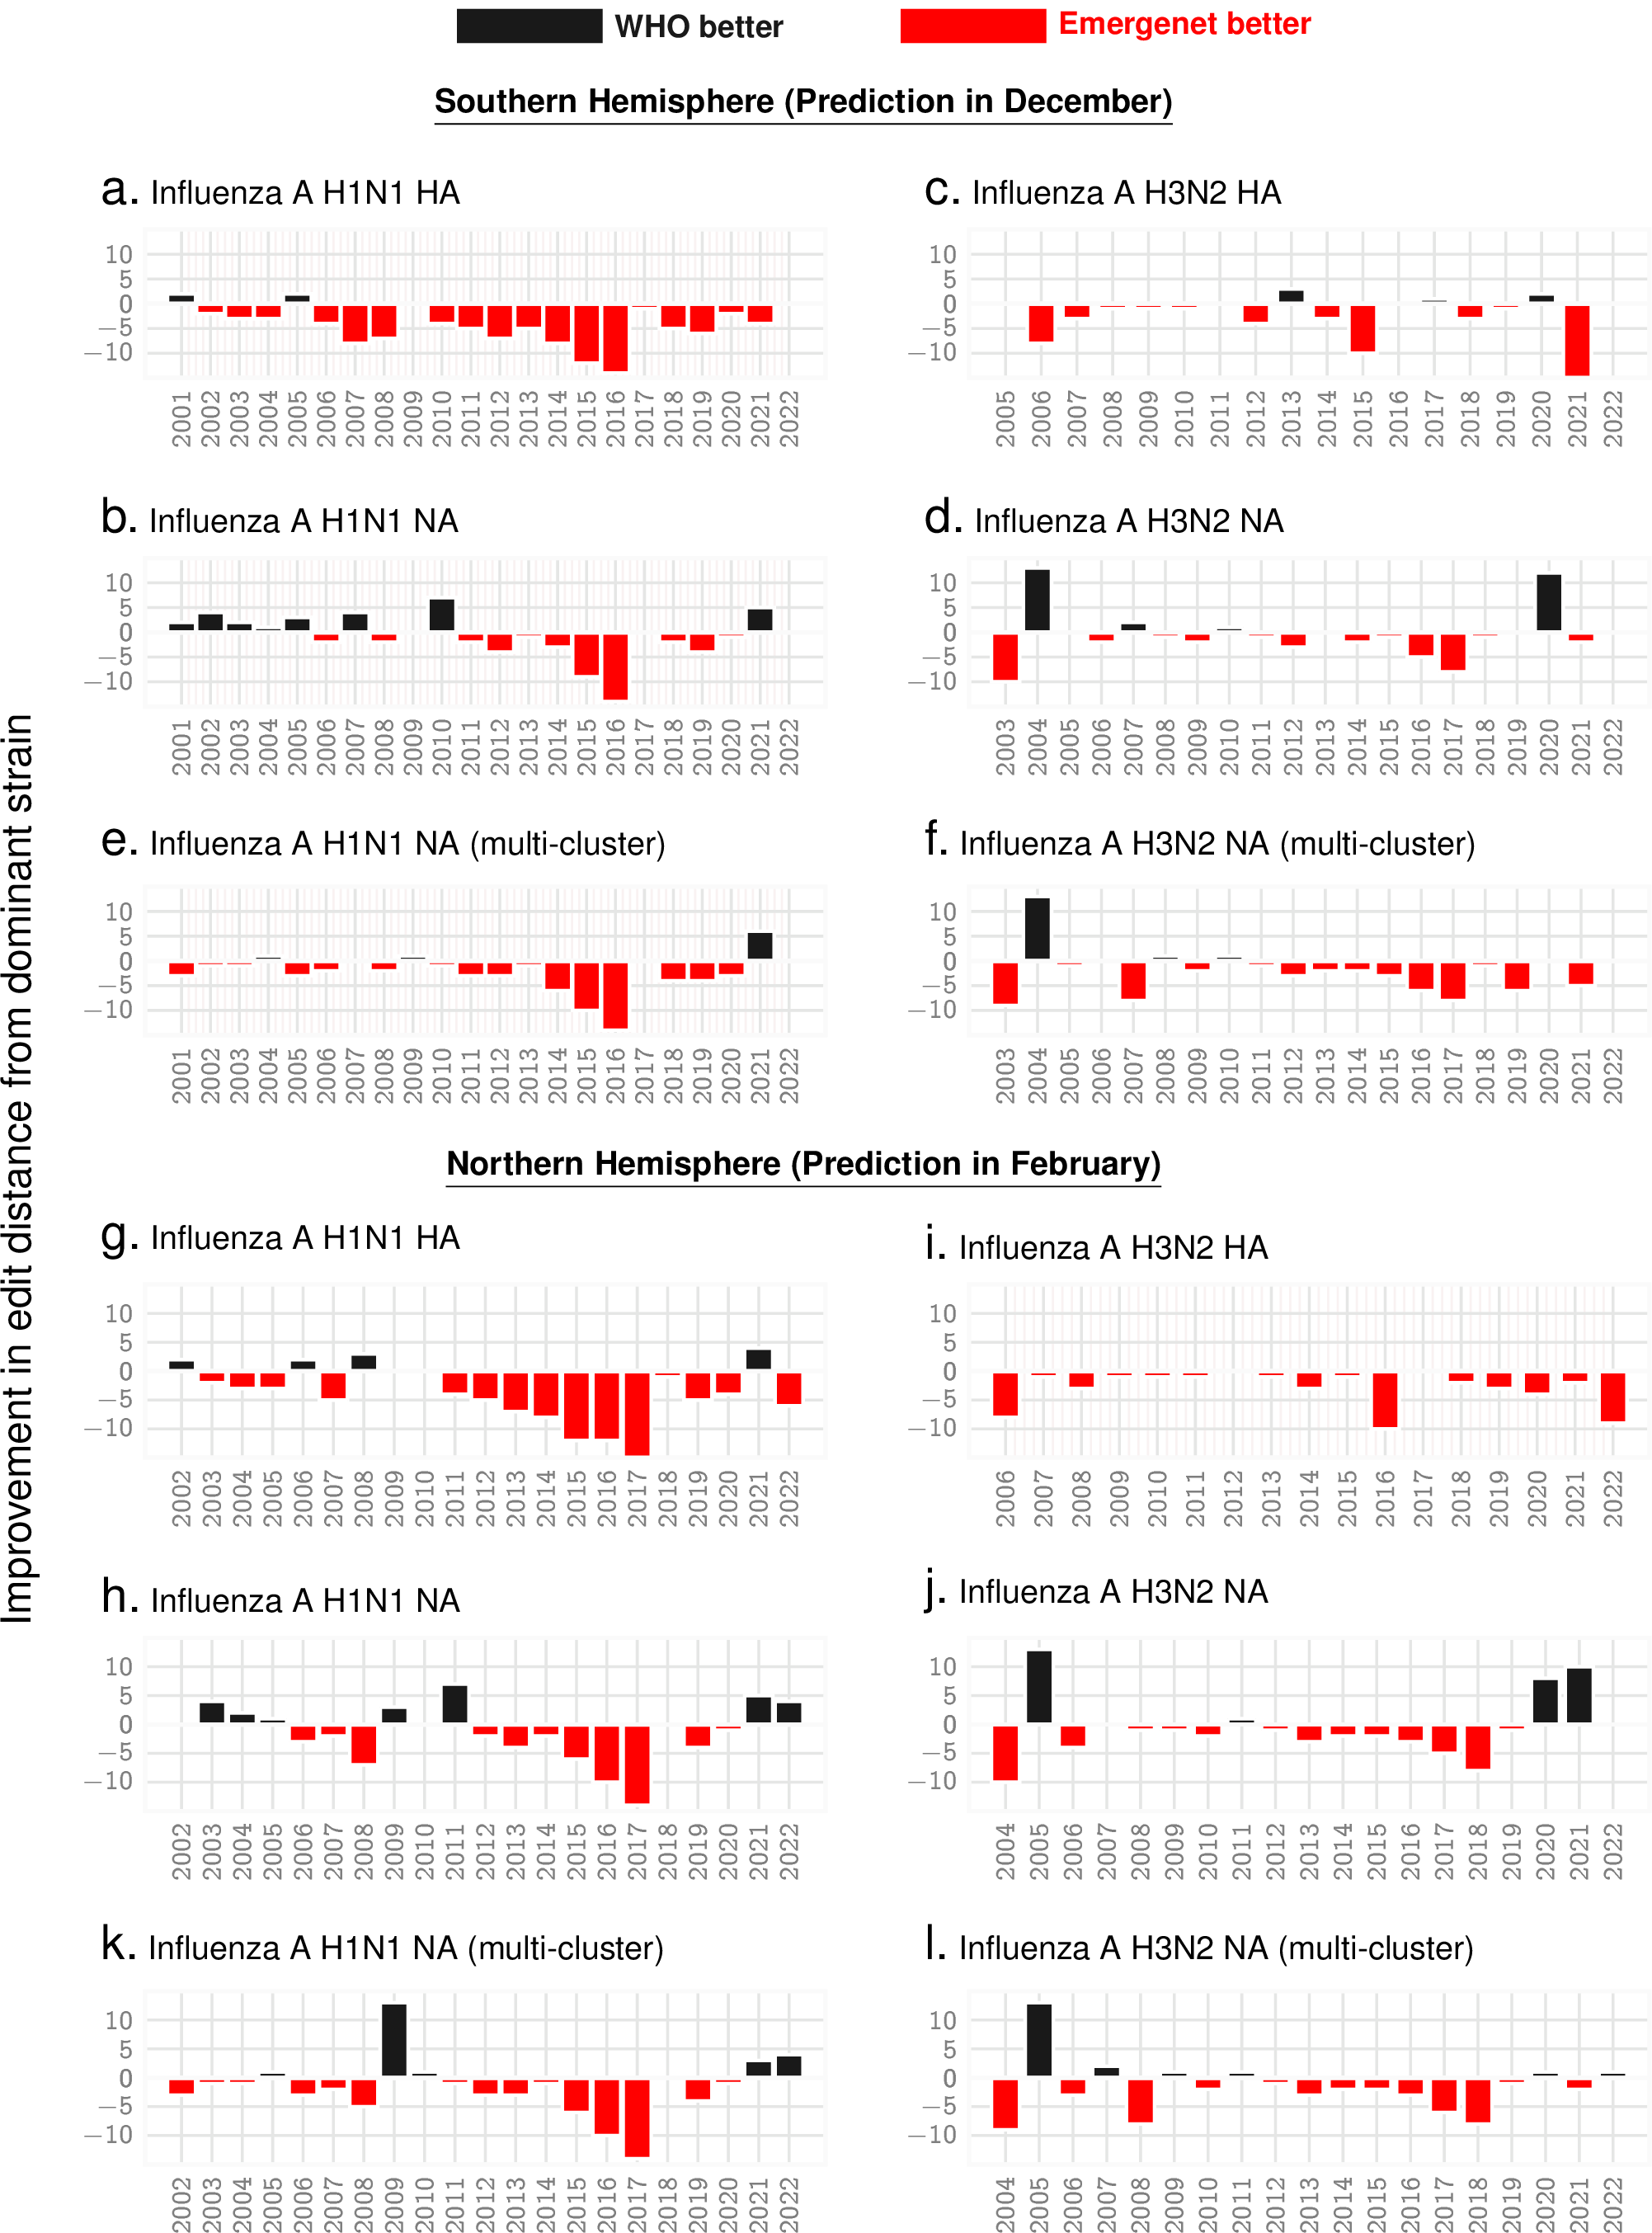
\includegraphics[width=0.975\textwidth]{Figures/seasonalpred_both.tex}
   \fi
   \captionN{\textbf{Seasonal predictions for Influenza A.} Relative out-performance of \qnet predictions against WHO recommendations for H1N1 and H3N2 sub-types for the HA and NA coding sequences over the both hemispheres. The negative bars (red) indicate the reduced edit distance between the predicted sequence and the actual dominant strain that emerged that year. Note that the recommendations for the north are given in February, while that for the south are given at the previous December, keeping in mind that the flu season in the south begins a few months early (e.g. for the 2021-2022 flu season, southern data in the table is labelled `2021' and northern is labelled `2022'). \textbf{Panels e, f, k, l} show further possible improvement in NA predictions if we return three recommendations instead of one each year.}\label{figseasonal}
\end{figure*}
\else
\refstepcounter{figure}\label{figseasonal}
\fi
%#############################################
%#############################################





%#############################################
%#############################################
\ifFIGS
\begin{figure*}[!ht]
  \centering
  \tikzexternalenable
    \tikzsetnextfilename{sequence}
\vspace{-5pt}

  \iftikzX
  \begin{tikzpicture}[font=\bf\sffamily\fontsize{8}{8}\selectfont]
  \def\SEQAA{Figures/plotdata/seqanal/2019-2020h1n1_HA_north}
  \def\SEQA{Figures/plotdata/seqanal/2018-2019h1n1_HA_north}
  \def\SEQB{Figures/plotdata/seqanal/2018-2019h1n1_HA_north}
  \def\SEQC{Figures/plotdata/seqanal/2016-2017h1n1_HA_north}
  \def\SEQD{Figures/plotdata/seqanal/2014-2015h1n1_HA_south}
  %\def\SEQCC{Figures/plotdata/seqanal/2016-2017h1n1_HA_south}
  \def\SEQE{Figures/plotdata/seqanal/2015-2016h3n2_HA_north}
  \def\LENA{550}
  \def\LENB{63}
  \def\LENC{286}
  \def\LENE{63}
  \def\LEND{312}
  \def\COLM{jet}
  \def\rndfileA{rndfile1.png}
  \def\rndfileB{rndfile2.png}
  \def\rndfileC{rndfile3.png}
  
  \newcommand{\panelX}[2] {
    \begin{tikzpicture}[font=\bf\sffamily\fontsize{7}{7}\selectfont]
      \node[ ] (A) at (0,0) {
        \mnp{3.2in}{\begin{texshade}{#1}
            %\shadingmode[chemical]{functional}
            \shadingmode[accessible area]{functional}
            \hideallmatchpositions
            \rulersteps{1}
            \setfont{residues}{sf}{up}{bf}{tiny} 
            \setfont{numbering}{sf}{up}{bf}{tiny} 
            \setfont{names}{tt}{up}{bf}{small}
            \setfont{legend}{tt}{up}{bf}{scriptsize}
            \threshold[80]{50}
            \setends{1}{1..\LENA}
            \showruler{1}{top}
            \hideconsensus
            \shadeallresidues
            #2
          \end{texshade}}};
\node[] (B) at (A.north east) {  \mnp{3.5in}{      
          % 
          \begin{texshade}{#1}
            %\shadingmode[standard area]{functional}
            \shadingmode[hydropathy]{functional}
            \hideallmatchpositions
            \rulersteps{1}
            \setfont{residues}{sf}{up}{bf}{tiny} 
            \setfont{numbering}{sf}{up}{bf}{tiny} 
            \setfont{names}{tt}{up}{bf}{small}
            \setfont{legend}{tt}{up}{bf}{scriptsize}
            \threshold[80]{50}
            \setends{1}{1..\LENA}
            \showruler{1}{top}
            \hideconsensus
            \shadeallresidues
            #2
          \end{texshade}}};
    \end{tikzpicture}
    }

  \clip (-2.4in,-7.35in) rectangle (4.4in,1.95in);
  \node[] (T1) at (0,0){  
    % 
    \begin{tikzpicture}
      \node[,label={[yshift=-.2in]90:{\large \sffamily \normalfont a.} 2018-2019 (H1N1 HA Northern Hemisphere)}]
      (A) at (0,0.0) {
        \mnp{.695\textwidth}{
          \begin{texshade}{\SEQA}
            \shadingmode[allmatchspecial]{identical}
            \shadingcolors{grays}
            \conservedresidues{White}{Red}{upper}{bf}
            \allmatchresidues{gray!50}{lightgray!10}{upper}{bf}
            \nomatchresidues{black}{lightgray!10}{upper}{bf}
            \setfont{residues}{sf}{up}{bf}{tiny} 
            \setfont{numbering}{sf}{up}{bf}{tiny} 
            \setfont{names}{tt}{up}{bf}{small}
            \setfont{legend}{tt}{up}{bf}{scriptsize}
            \setfont{features}{tt}{up}{bf}{scriptsize}
            \feature{top}{1}{\LENB..\LENC}{brace[black]}{RBD}
            % \threshold[80]{50}
            \setends{1}{\LENE..\LEND}
            \showruler{1}{top}
            \hideconsensus
            % \defconsensus{.}{lower}{upper}
            % \showlegend
          \end{texshade}
          % 
        }};
    \end{tikzpicture}};

 \node[anchor=north west,label={[yshift=-.1in]90:{\large \large \sffamily \normalfont b.} 2019-2020 (H1N1 HA Northern Hemisphere)}] (T21) at ([xshift=-0.08in]T1.south west) {\panelX{\SEQAA}{}};

 \node[anchor=north west,label={[xshift=-.05in,yshift=-.05in]90:{\large \large \sffamily \normalfont c.} 2018-2019 (H1N1 HA Northern Hemisphere)}] (T2) at ([xshift=-0.0in]T21.south west) {\panelX{\SEQB}{}};

 \node[anchor=north west,label={[xshift=-.05in,yshift=-.05in]90:{\large \large \sffamily \normalfont d.} 2016-2017 (H1N1 HA Northern Hemisphere)}] (T3) at ([xshift=-0.0in]T2.south west) {\panelX{\SEQC}{}};

 \node[anchor=north west,label={[xshift=-.05in,yshift=-.05in]90:{\large \large \sffamily \normalfont e.} 2014-2015 (H1N1 HA Southern Hemisphere)}] (T4) at ([xshift=-0.0in]T3.south west) {\panelX{\SEQD}{}};

 \node[anchor=north west,label={[xshift=-.1in,yshift=-.05in]90:{\large \large \sffamily \normalfont f.} 2015-2016 (H3N2 HA Northern Hemisphere)}] (T5) at ([xshift=-0.0in]T4.south west) {\panelX{\SEQE}{\showlegend}};


 \node[anchor=north west] (T11) at ([xshift=-.45in,yshift=0.15in]T1.north east) {
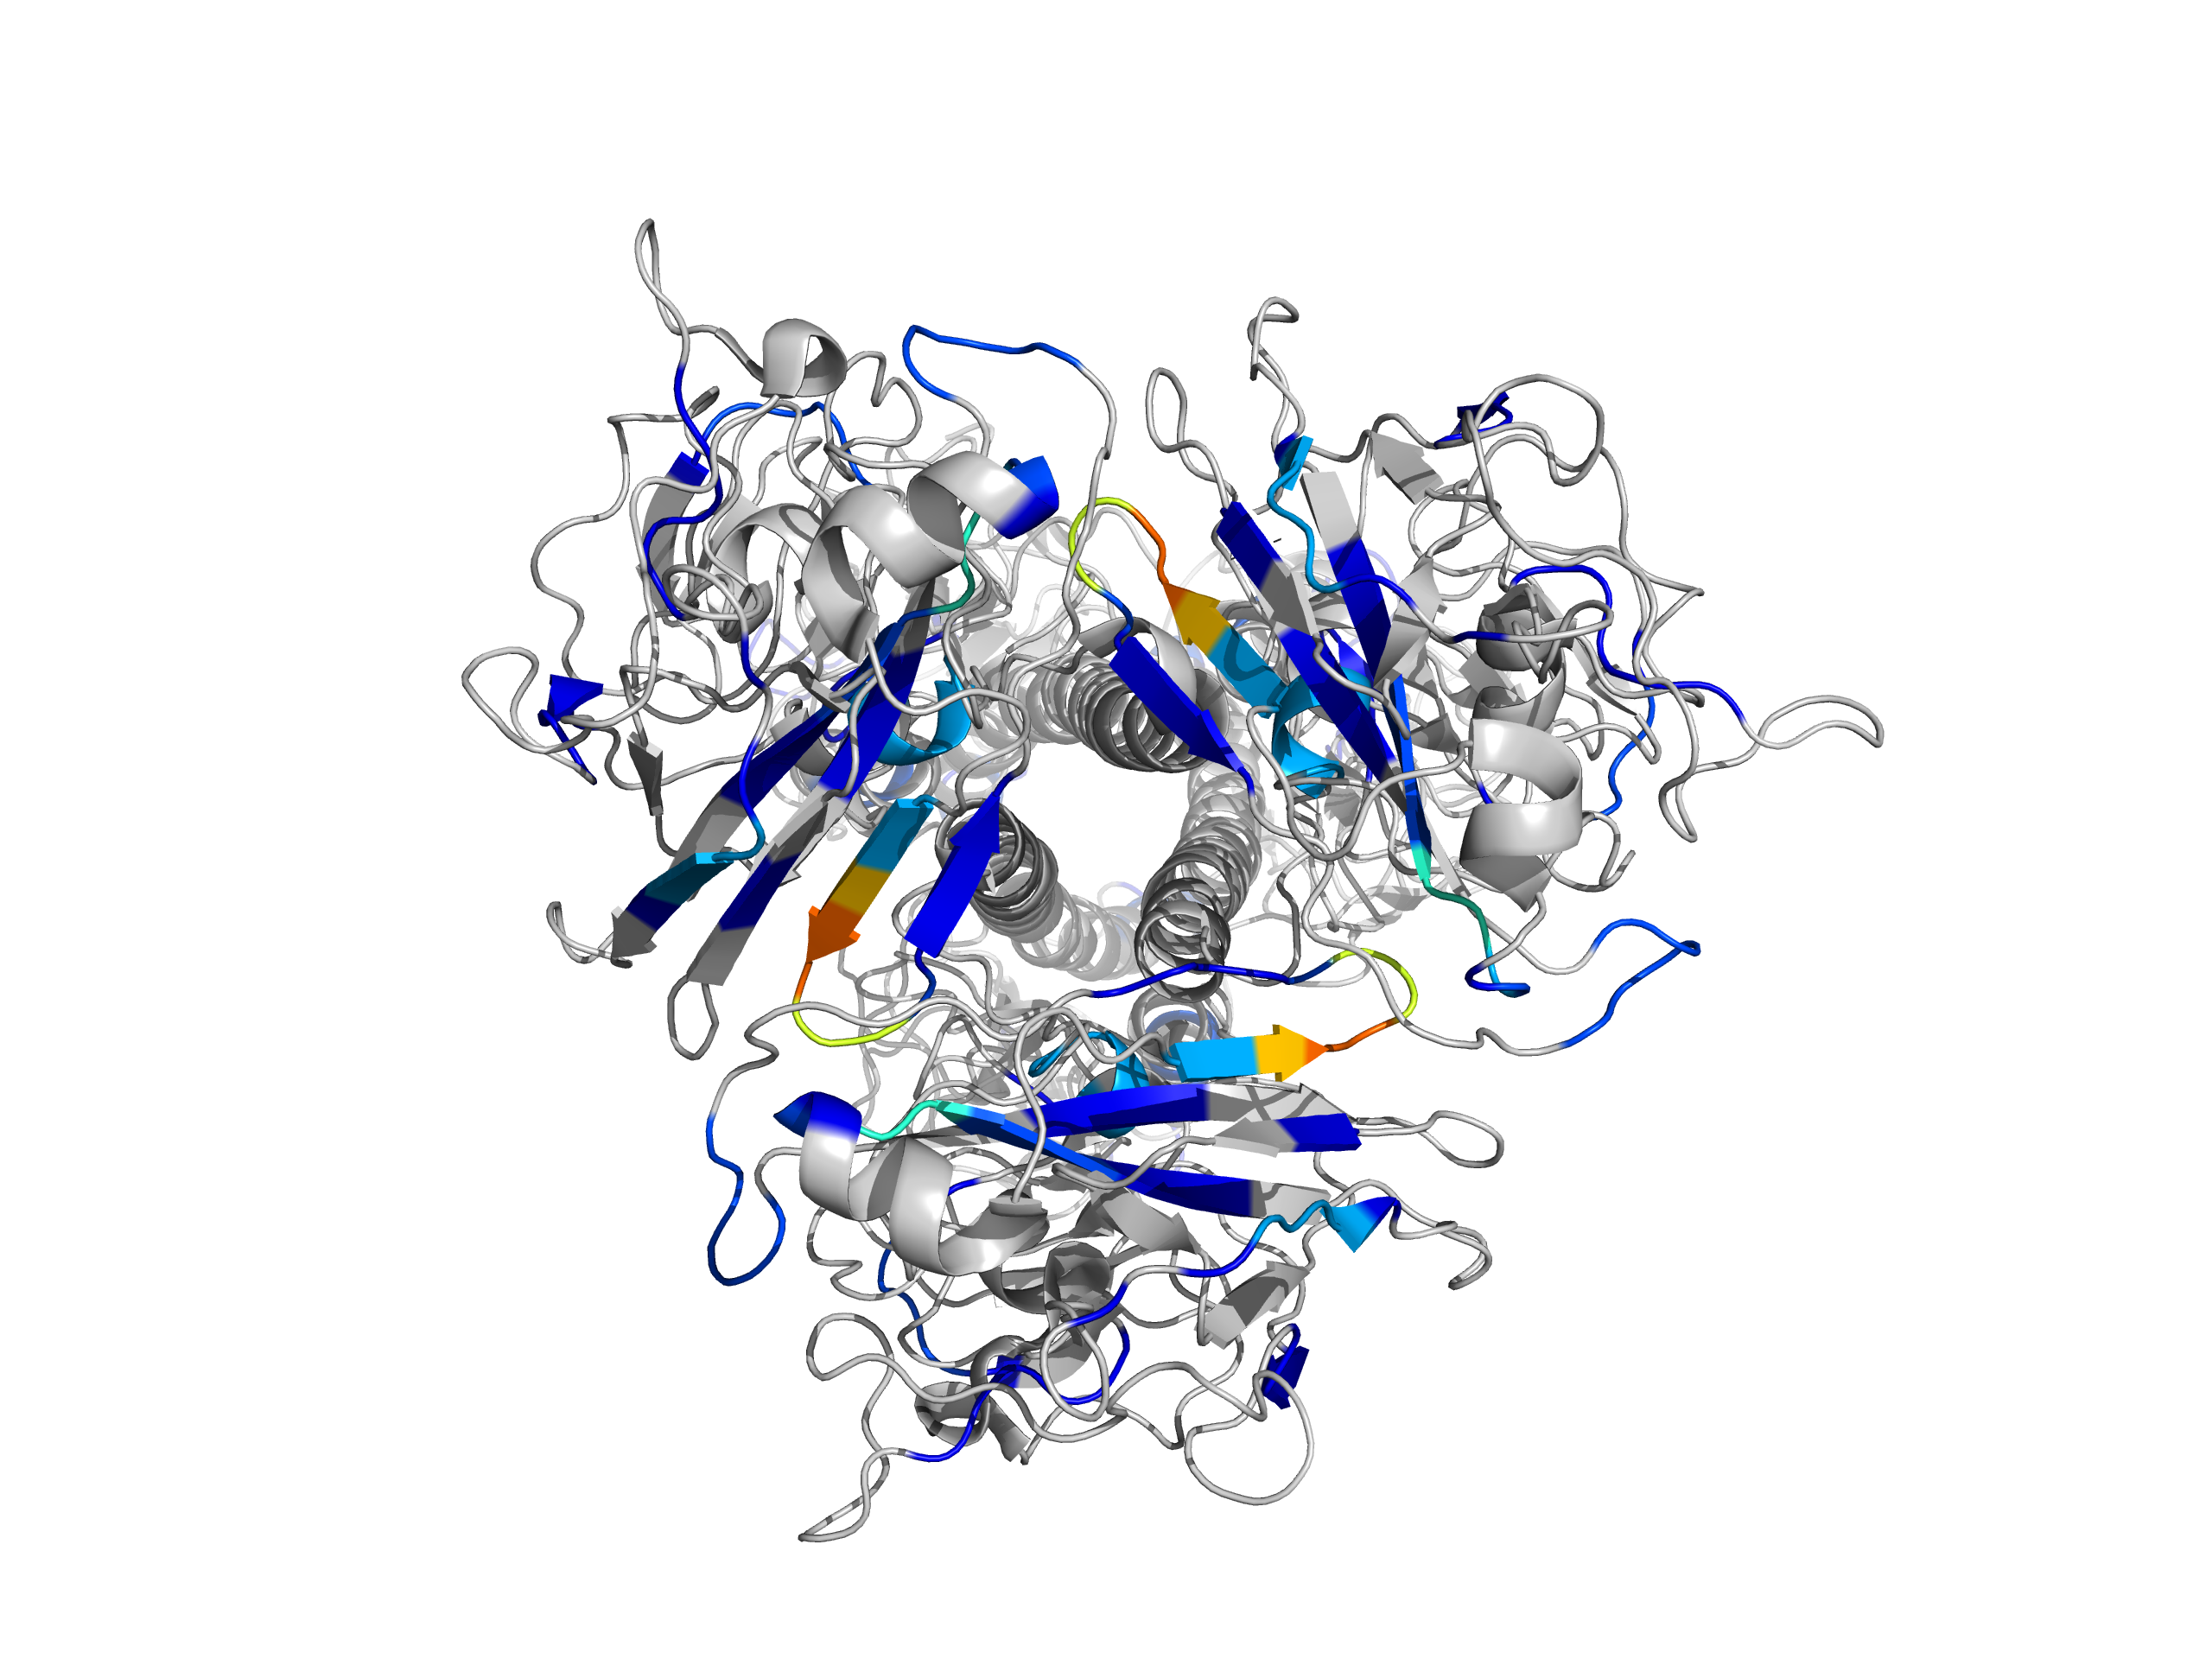
\includegraphics[width=2.75in]{/home/ishanu/ZED/Research/publications/pub_pan_one_/Figures/plotdata/seqanal/ntb/jetrndfile1.png}};
 \node[anchor=north west] (T111) at ([yshift=-0.15in,xshift=0.05in]T11.south west) {
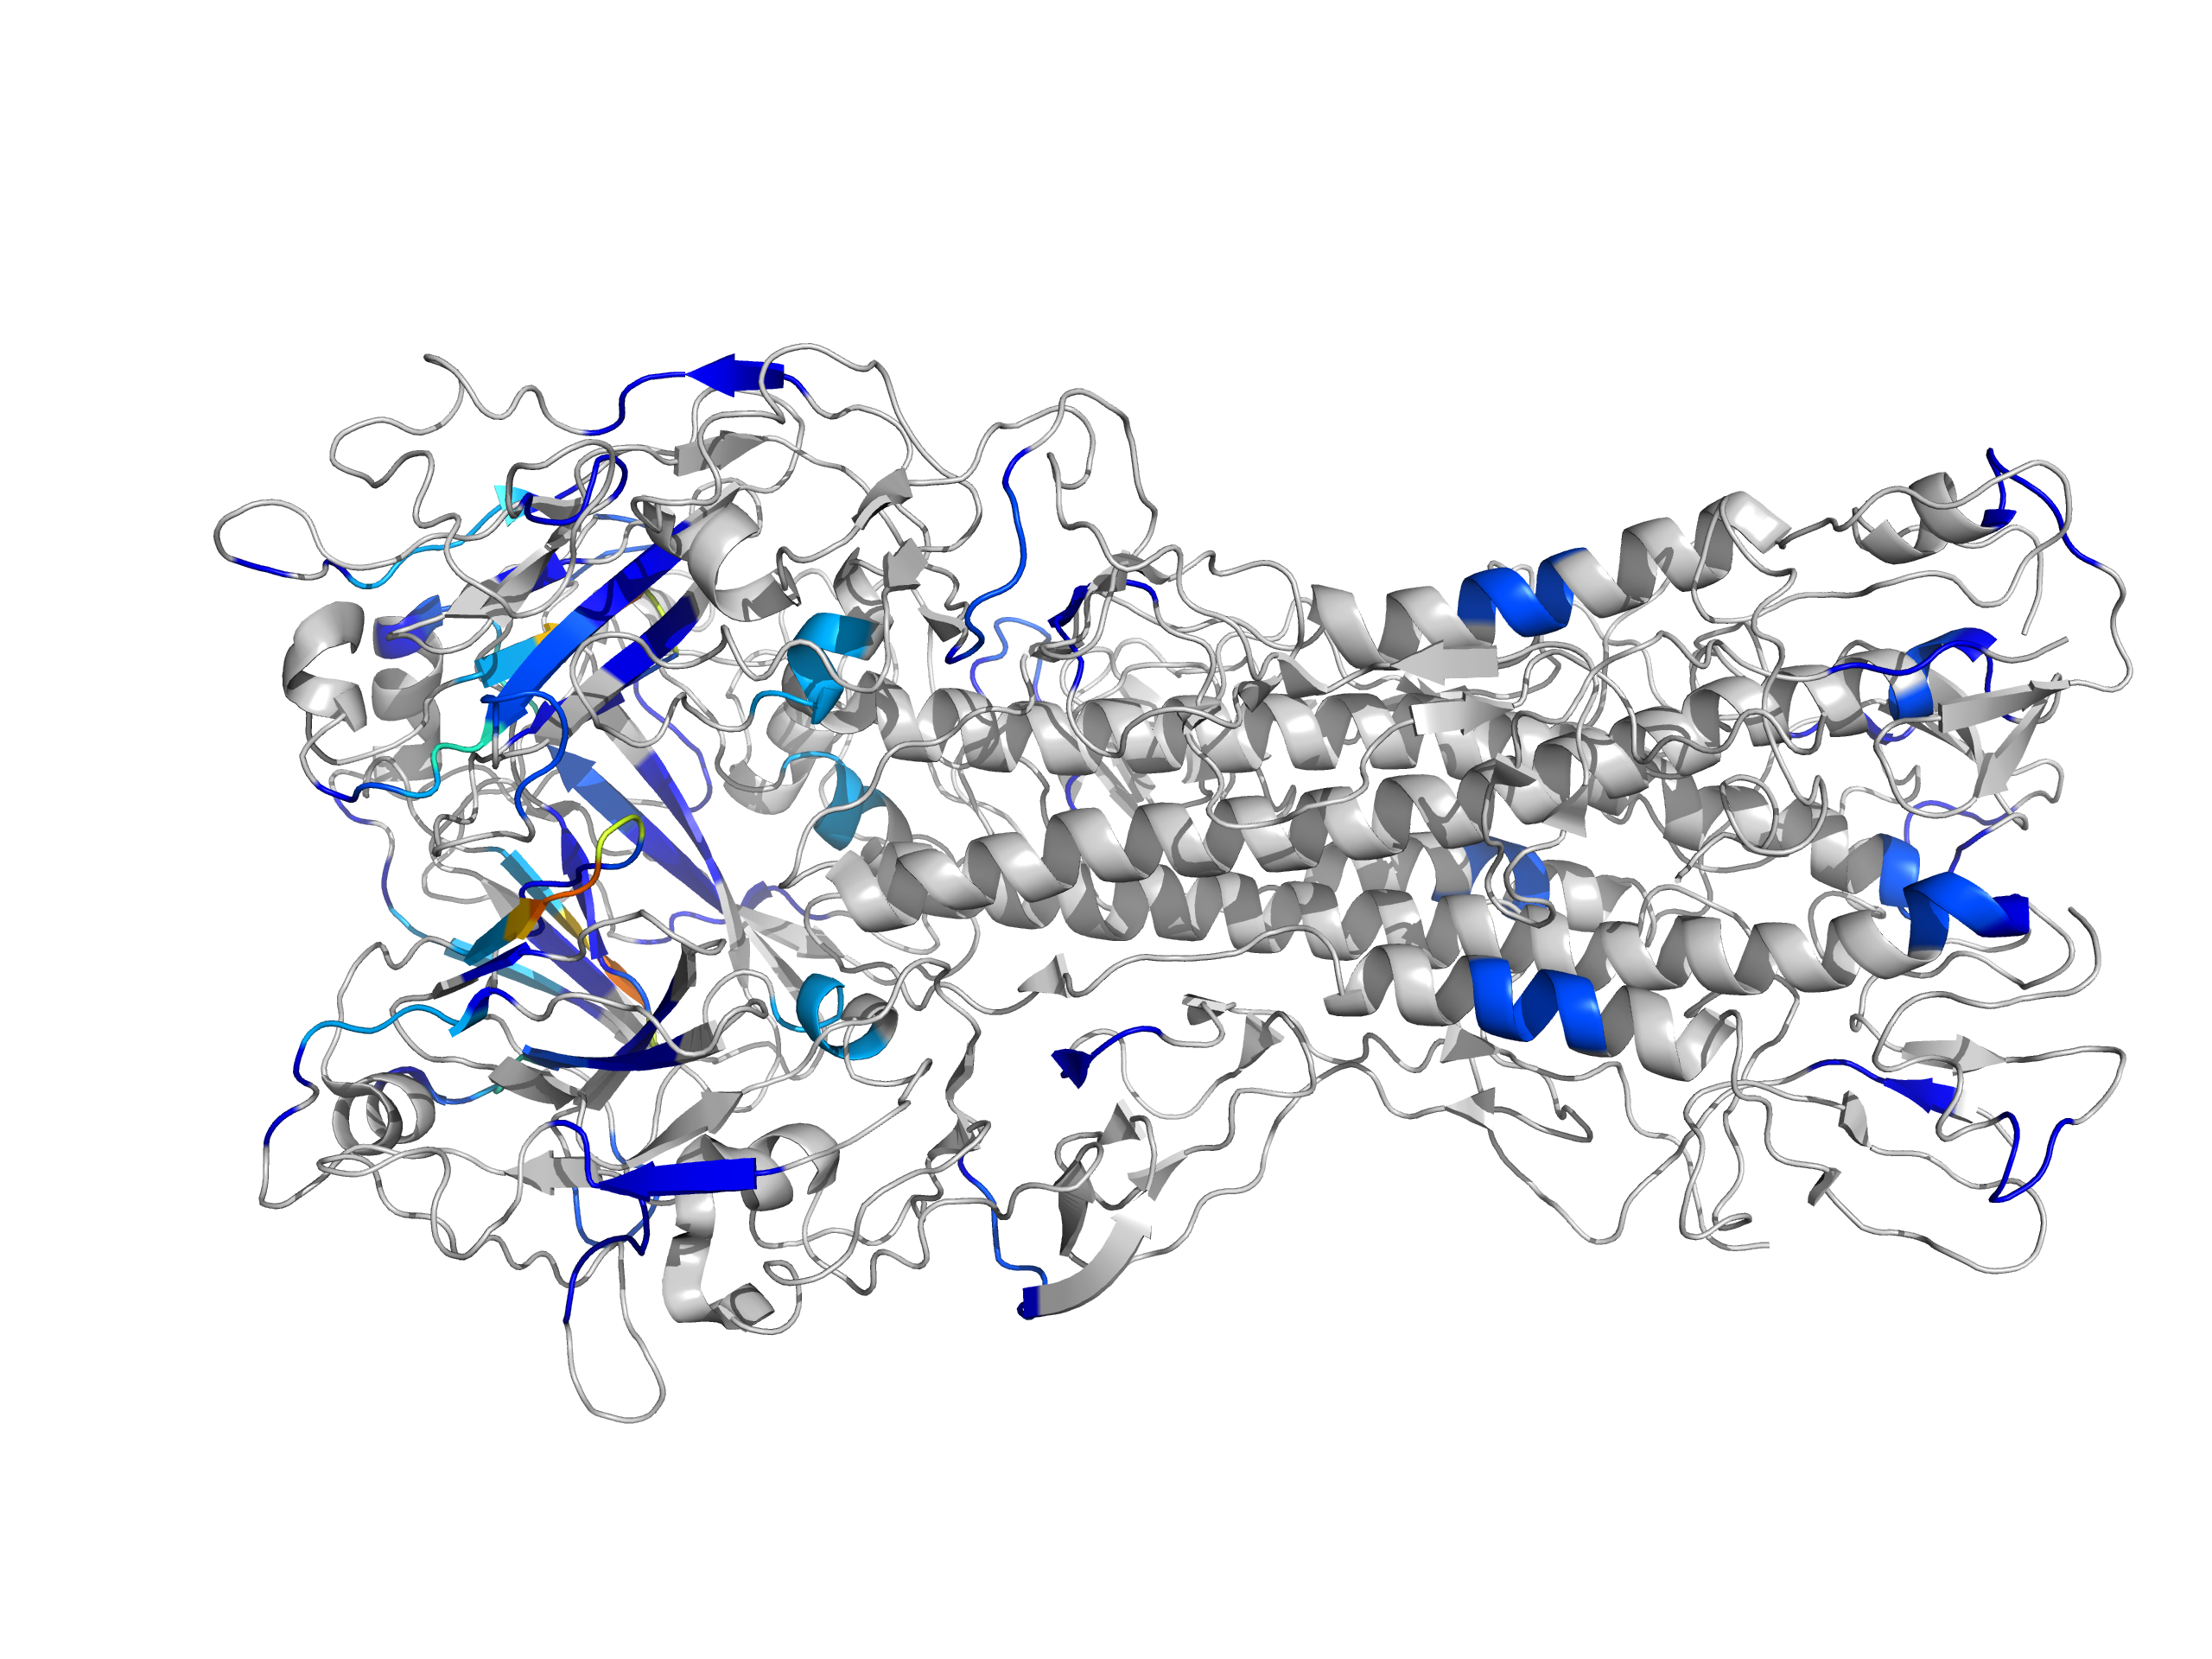
\includegraphics[width=3.5in,angle=-90]{/home/ishanu/ZED/Research/publications/pub_pan_one_/Figures/plotdata/seqanal/ntb/jetrndfile2.png}};
 \node[anchor=north west] (T112) at ([yshift=0.2in,xshift=.86in]T11.south west) {
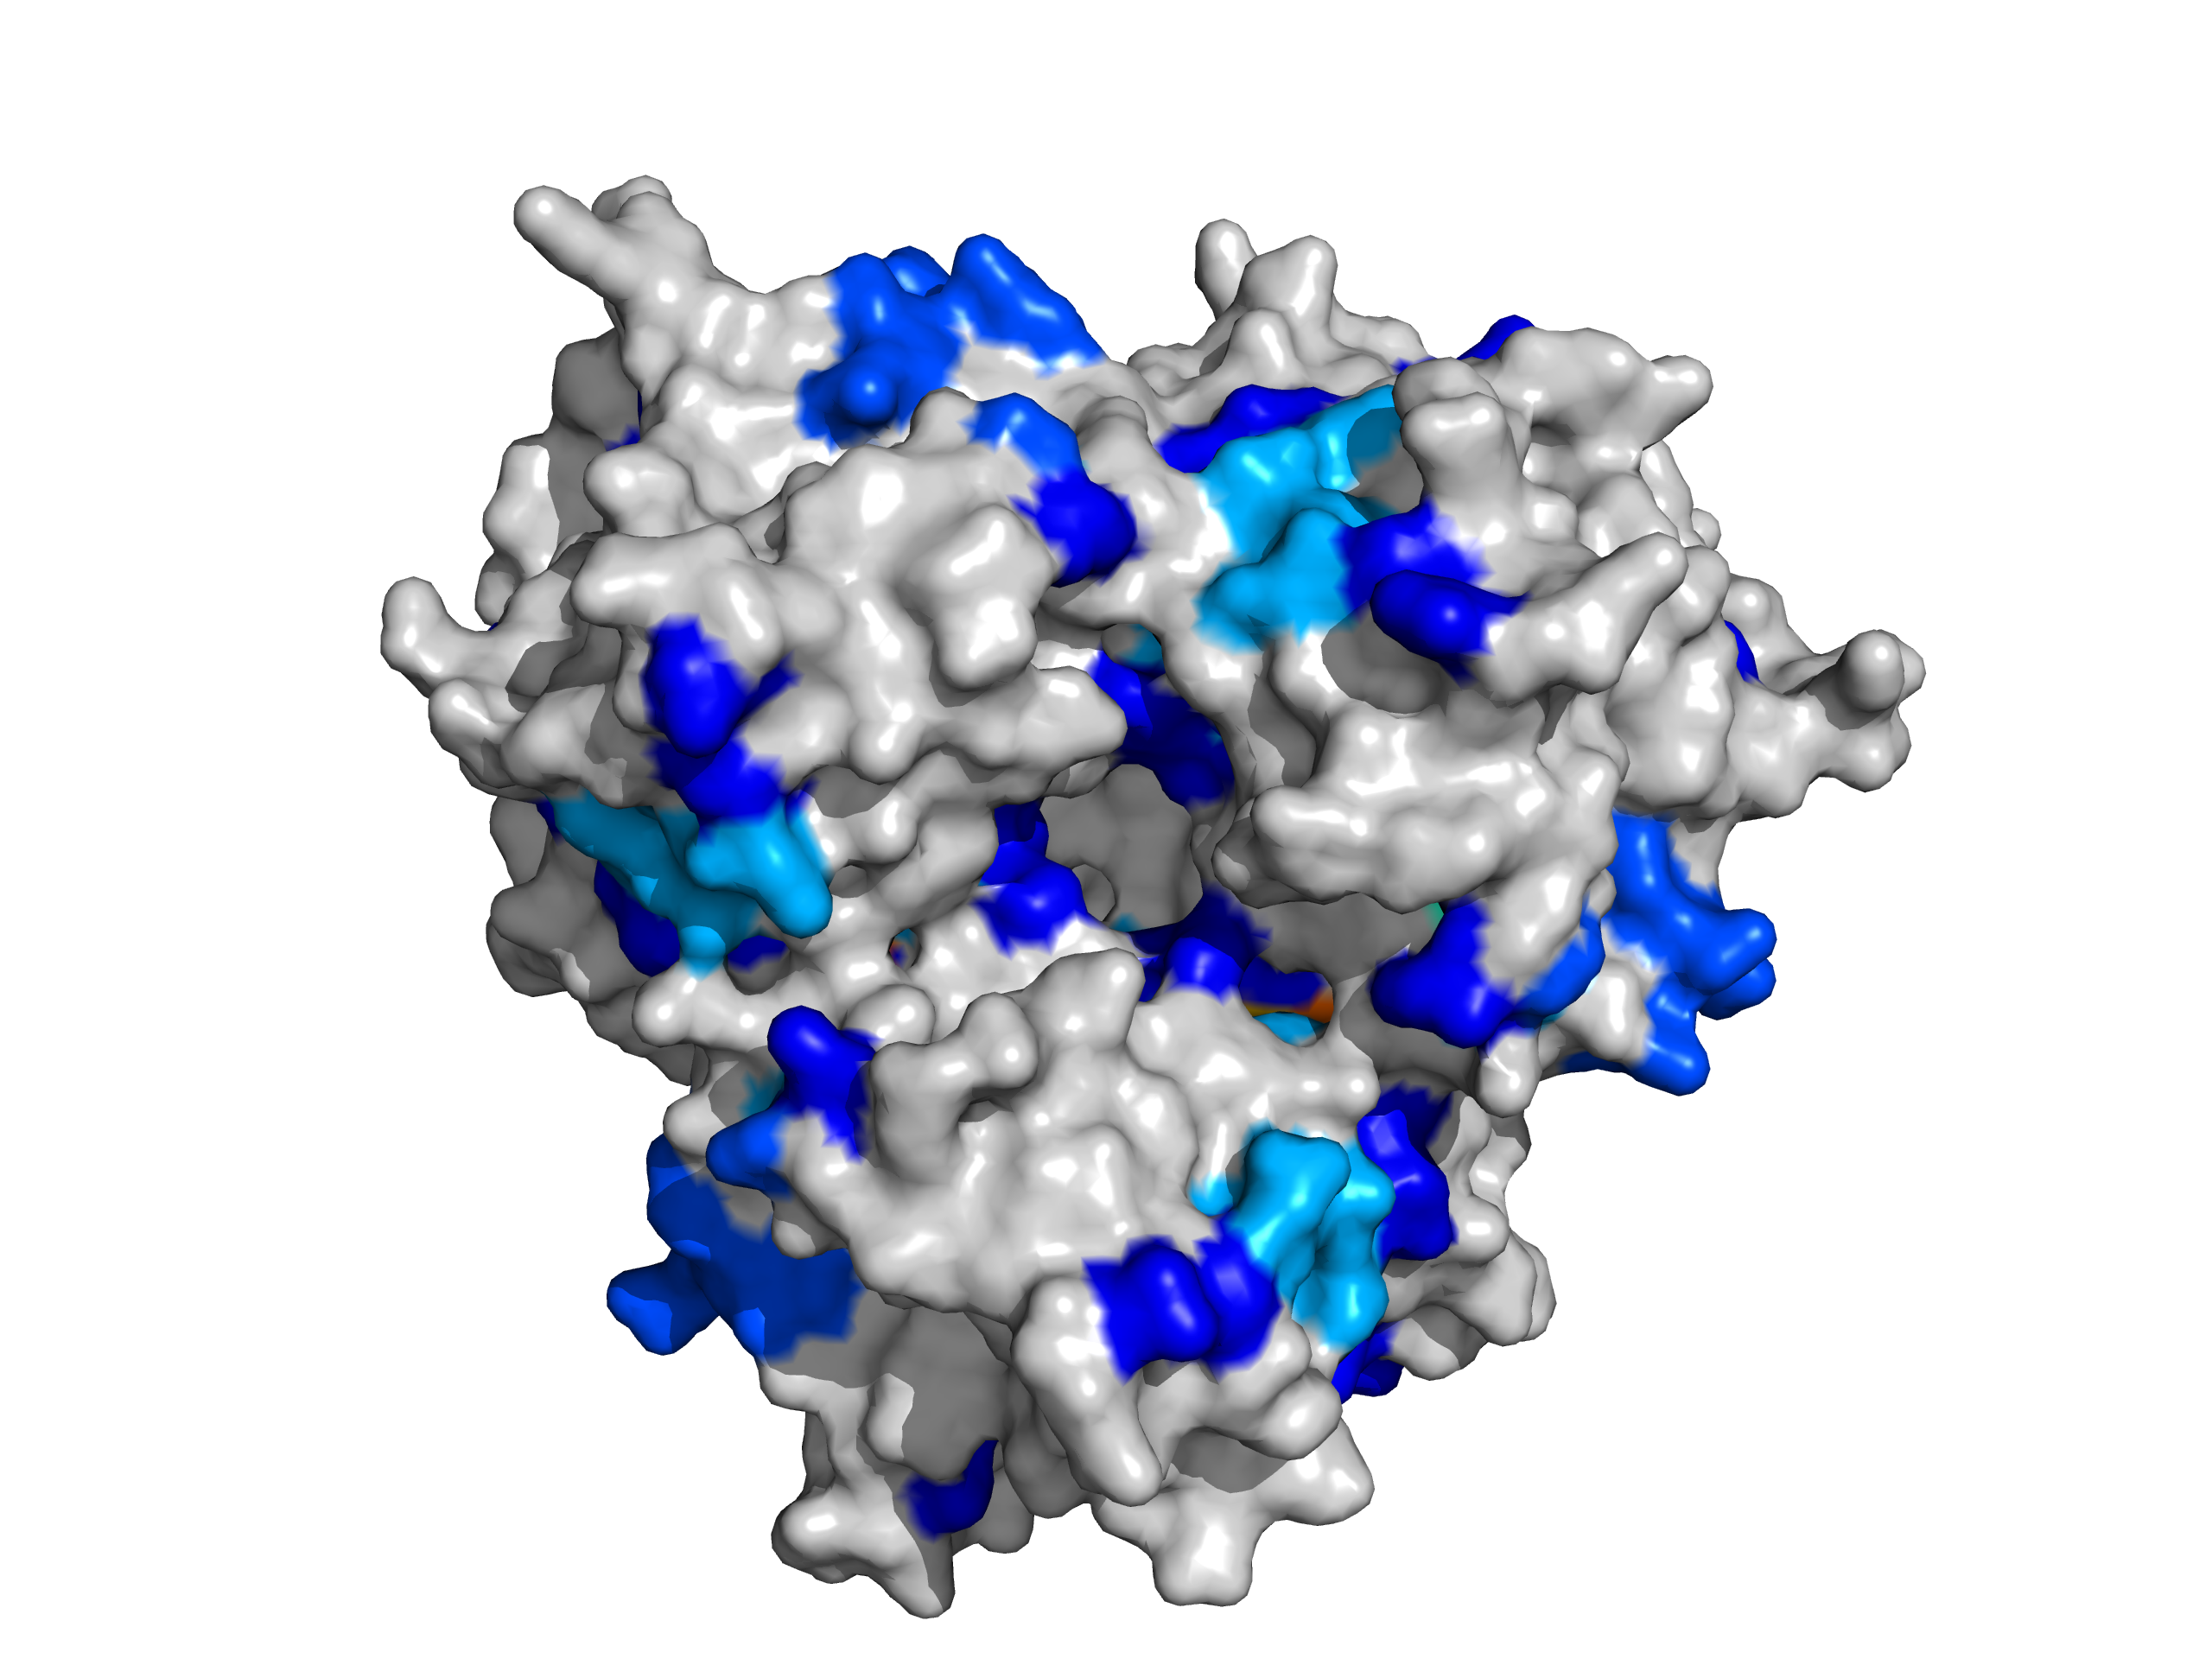
\includegraphics[width=1in]{/home/ishanu/ZED/Research/publications/pub_pan_one_/Figures/plotdata/seqanal/ntb/jetrndfile4.png}};
   

 \node[anchor=north west] (L2) at ([xshift=.6in,yshift=-0.05in]$(T1.north west)!(T11.west)!(T1.north east)$) {{\large \normalfont g.}};
 \node[anchor=north west] (L3) at ([xshift=.6in,yshift=-.1in]$(T11.north west)!(T112.north)!(T11.south west)$) {{\large \normalfont h.}};
 \node[anchor=north west] (L4) at ([xshift=.6in,yshift=-.45in]$(T11.north west)!(T111.north)!(T11.south west)$) {{\large \normalfont i.}};

\draw [thin, dashed] (T11.center) -- (T111.center);
\draw [-{latex},thin,Red1] ([xshift=-.8in,yshift=-.5in]T11.center) -- ([xshift=-.38in,yshift=-.17in]T11.center) node [pos=0.1,xshift=-.15in,yshift=-.02in,font=\bf\sffamily\fontsize{6}{6}\selectfont,text=black] {200} ;
\draw [-{latex},thin,Red1] ([xshift=-.8in,yshift=-.5in]T11.center) -- ([xshift=-0.12in,yshift=-2.1in]T11.center);
\draw [-{latex},thin,Red1] ([xshift=.6in,yshift=-.65in]T11.center) -- ([xshift=.3in,yshift=-.29in]T11.center) node [pos=-0.15,font=\bf\sffamily\fontsize{6}{6}\selectfont,text=black,fill=white] {200};
\draw [-{latex},thin,Red1] ([xshift=.1in,yshift=.7in]T11.center) -- ([xshift=.1in,yshift=.34in]T11.center) node [pos=-0.15,font=\bf\sffamily\fontsize{6}{6}\selectfont,text=black,fill=white] {200};

\draw [-{latex},thin,Red1] ([xshift=.73in,yshift=-.45in]T11.center) -- ([xshift=.7in,yshift=-.2in]T11.center) node [pos=-0.15,font=\bf\sffamily\fontsize{6}{6}\selectfont,text=black,fill=white] {220};

\draw [-{latex},thin,Red1] ([xshift=.73in,yshift=-.45in]T11.center) -- ([xshift=.7in,yshift=-.2in]T11.center) node [pos=-0.15,font=\bf\sffamily\fontsize{6}{6}\selectfont,text=black,fill=white] {220};

\draw [-{latex},thin,Red1] ([xshift=.53in,yshift=-.35in]T11.center) -- ([xshift=.42in,yshift=-0.1in]T11.center) node [pos=-0.15,font=\bf\sffamily\fontsize{6}{6}\selectfont,text=black] {180};

\draw [-{latex},thin,Red1] ([xshift=.53in,yshift=-.35in]T111.center) -- ([xshift=.42in,yshift=-0.6in]T111.center) node [pos=-0.15,xshift=.05in,font=\bf\sffamily\fontsize{6}{6}\selectfont,text=black] {49(HA2)};

\draw [-{latex},thin,Red1] ([xshift=-.8in,yshift=-.15in]T111.center) -- ([xshift=-.35in,yshift=0.4in]T111.center) node [pos=-0.15,xshift=.05in,font=\bf\sffamily\fontsize{6}{6}\selectfont,text=black] {100};

\draw [-{latex},thin,Red1] ([xshift=-1in,yshift=.2in]T111.center) -- ([xshift=-.6in,yshift=0.65in]T111.center) node [pos=-0.15,xshift=.05in,font=\bf\sffamily\fontsize{6}{6}\selectfont,text=black] {115};

\draw [-{latex},thin,Red1] ([xshift=-.8in,yshift=-1.1in]T111.center) -- ([xshift=-0.1in,yshift=-1.32in]T111.center) node [pos=-0.15,xshift=.05in,yshift=.01in,font=\bf\sffamily\fontsize{6}{6}\selectfont,text=black] {124 (HA2)};

\node[fill=white,  opacity=.65] (CC) at ([xshift=.1in,yshift=.02in]T112.east) {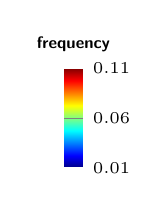
\begin{tikzpicture}
\begin{axis}[font=\bf\sffamily\fontsize{6}{6}\selectfont,
  hide axis,major tick length=0pt,
  xtick=\empty,
    scale only axis,
    height=0pt,
    width=0pt,
    colormap/jet,
    colorbar,
    point meta min=0.01,
    point meta max=0.11,
    colorbar style={title={frequency},title style={yshift=-.05in},font=\bf\sffamily\fontsize{6}{6}\selectfont,draw=none,axis line style={white}, y tick label style={
        /pgf/number format/.cd,
            fixed,
            fixed zerofill,
            precision=2,
        /tikz/.cd
    },  height=.5in,width=.1in,
        ytick={0.01,0.06,0.11}
    }]
    \addplot [draw=none] coordinates {(0,0)};
\end{axis}
\end{tikzpicture}};
  % \node[anchor=north west,label={[]90:{\large b.} 2018-2019 (Northern Hemisphere)}] (T2) at ([xshift=.1in]T1.south west) {
  %   \begin{tikzpicture}[font=\bf\sffamily\fontsize{7}{7}\selectfont]
  %     \node[] (A) at (0,0) {
  %       \mnp{2.65in}{\begin{texshade}{\SEQB}
  %           \shadingmode[chemical]{functional}
  %           \hideallmatchpositions
  %           \rulersteps{1}
  %           \setfont{residues}{sf}{up}{bf}{tiny} 
  %           \setfont{numbering}{sf}{up}{bf}{tiny} 
  %           \setfont{names}{tt}{up}{bf}{small}
  %           \setfont{legend}{tt}{up}{bf}{scriptsize}
  %           \threshold[80]{50}
  %           \setends{1}{1..\LENA}
  %           \showruler{1}{top}
  %           \hideconsensus
  %           \shadeallresidues
  %           \showlegend
  %         \end{texshade}
  %         % 
  %         \begin{texshade}{\SEQB}
  %           %\shadingmode[standard area]{functional}
  %           \shadingmode[hydropathy]{functional}
  %           \hideallmatchpositions
  %           \rulersteps{1}
  %           \setfont{residues}{sf}{up}{bf}{tiny} 
  %           \setfont{numbering}{sf}{up}{bf}{tiny} 
  %           \setfont{names}{tt}{up}{bf}{small}
  %           \setfont{legend}{tt}{up}{bf}{scriptsize}
  %           \threshold[80]{50}
  %           \setends{1}{1..\LENA}
  %           \showruler{1}{top}
  %           \hideconsensus
  %           \shadeallresidues
  %           \showlegend
  %         \end{texshade}
  %         % 
  %         \begin{texshade}{\SEQB}
  %           \shadingmode[accessible area]{functional}
  %           \hideallmatchpositions
  %           \rulersteps{1}
  %           \setfont{residues}{sf}{up}{bf}{tiny}
  %           \setfont{numbering}{sf}{up}{bf}{tiny} 
  %           \setfont{names}{tt}{up}{bf}{small}
  %           \setfont{legend}{tt}{up}{bf}{scriptsize}
  %           \threshold[80]{50}
  %           \setends{1}{1..\LENA}
  %           \showruler{1}{top}
  %           \hideconsensus
  %           \shadeallresidues
  %           \showlegend
  %         \end{texshade}
  %         % 
  %       }};
  %   \end{tikzpicture}};

 %  \node[anchor=north west,label={[]90:{\large c.} 2016-2017 (Southern Hemisphere)}] (T2) at ([xshift=0in]T1.south west) {
%     \begin{tikzpicture}[font=\bf\sffamily\fontsize{7}{7}\selectfont]
%       \node[ ] (A) at (0,0) {
%         \mnp{3.5in}{\begin{texshade}{\SEQC}
%             %\shadingmode[chemical]{functional}
%             \shadingmode[accessible area]{functional}
%             \hideallmatchpositions
%             \rulersteps{1}
%             \setfont{residues}{sf}{up}{bf}{tiny} 
%             \setfont{numbering}{sf}{up}{bf}{tiny} 
%             \setfont{names}{tt}{up}{bf}{small}
%             \setfont{legend}{tt}{up}{bf}{scriptsize}
%             \threshold[80]{50}
%             \setends{1}{1..\LENA}
%             \showruler{1}{top}
%             \hideconsensus
%             \shadeallresidues
%             \showlegend
%           \end{texshade}}};
% \node[] (B) at (A.north east) {  \mnp{3.5in}{      
%           % 
%           \begin{texshade}{\SEQC}
%             %\shadingmode[standard area]{functional}
%             \shadingmode[hydropathy]{functional}
%             \hideallmatchpositions
%             \rulersteps{1}
%             \setfont{residues}{sf}{up}{bf}{tiny} 
%             \setfont{numbering}{sf}{up}{bf}{tiny} 
%             \setfont{names}{tt}{up}{bf}{small}
%             \setfont{legend}{tt}{up}{bf}{scriptsize}
%             \threshold[80]{50}
%             \setends{1}{1..\LENA}
%             \showruler{1}{top}
%             \hideconsensus
%             \shadeallresidues
%             \showlegend
%           \end{texshade}}};


      
%     \end{tikzpicture}};


  

  % \node[anchor=north west,label={[]90:{\large d.} 2016-2017 (Northern Hemisphere)}] (T4) at ([xshift=0in]T3.south west) {
  %   \begin{tikzpicture}[font=\bf\sffamily\fontsize{7}{7}\selectfont]
  %     \node[label={[yshift=-1in,xshift=.15in]170:\mnp{.4in}{\raggedright type \\ \vspace{35pt} sd. chn. area \\ \vspace{35pt} acc. sd. chn.}}] (A) at (0,0) {
  %       \mnp{3.2in}{\begin{texshade}{\SEQD}
  %           \shadingmode[chemical]{functional}
  %           \hideallmatchpositions
  %           \rulersteps{1}
  %           \setfont{residues}{sf}{up}{bf}{tiny} 
  %           \setfont{numbering}{sf}{up}{bf}{tiny} 
  %           \setfont{names}{tt}{up}{bf}{small}
  %           \setfont{legend}{tt}{up}{bf}{scriptsize}
  %           \threshold[80]{50}
  %           \setends{1}{1..\LENA}
  %           \showruler{1}{top}
  %           \hideconsensus
  %           \shadeallresidues
  %           % \showlegend
  %         \end{texshade}
  %         % 
  %         \begin{texshade}{\SEQD}
  %           %\shadingmode[standard area]{functional}
  %           \shadingmode[hydropathy]{functional}
  %           \hideallmatchpositions
  %           \rulersteps{1}
  %           \setfont{residues}{sf}{up}{bf}{tiny} 
  %           \setfont{numbering}{sf}{up}{bf}{tiny} 
  %           \setfont{names}{tt}{up}{bf}{small}
  %           \setfont{legend}{tt}{up}{bf}{scriptsize}
  %           \threshold[80]{50}
  %           \setends{1}{1..\LENA}
  %           \showruler{1}{top}
  %           \hideconsensus
  %           \shadeallresidues
  %           % \showlegend
  %         \end{texshade}
  %         % 
  %         \begin{texshade}{\SEQD}
  %           \shadingmode[accessible area]{functional}
  %           \hideallmatchpositions
  %           \rulersteps{1}
  %           \setfont{residues}{sf}{up}{bf}{tiny}
  %           \setfont{numbering}{sf}{up}{bf}{tiny} 
  %           \setfont{names}{tt}{up}{bf}{small}
  %           \setfont{legend}{tt}{up}{bf}{scriptsize}
  %           \threshold[80]{50}
  %           \setends{1}{1..\LENA}
  %           \showruler{1}{top}
  %           \hideconsensus
  %           \shadeallresidues
  %           % \showlegend
  %         \end{texshade}
  %         % 
  %       }};
  %   \end{tikzpicture}};



  % \node[anchor=north west,label={[]90:{\large e.} 2016-2017 (H3N2 Northern Hemisphere)}] (T5) at ([xshift=0in]T4.south west) {
  %   \begin{tikzpicture}[font=\bf\sffamily\fontsize{7}{7}\selectfont]
  %     \node[label={[yshift=-1in,xshift=.15in]170:\mnp{.4in}{\raggedright type \\ \vspace{35pt} sd. chn. area \\ \vspace{35pt} acc. sd. chn.}}] (A) at (0,0) {
  %       \mnp{3.2in}{\begin{texshade}{\SEQE}
  %           \shadingmode[chemical]{functional}
  %           \hideallmatchpositions
  %           \rulersteps{1}
  %           \setfont{residues}{sf}{up}{bf}{tiny} 
  %           \setfont{numbering}{sf}{up}{bf}{tiny} 
  %           \setfont{names}{tt}{up}{bf}{small}
  %           \setfont{legend}{tt}{up}{bf}{scriptsize}
  %           \threshold[80]{50}
  %           \setends{1}{1..\LENA}
  %           \showruler{1}{top}
  %           \hideconsensus
  %           \shadeallresidues
  %           % \showlegend
  %         \end{texshade}
  %         % 
  %         \begin{texshade}{\SEQE}
  %           %\shadingmode[standard area]{functional}
  %           \shadingmode[hydropathy]{functional}
  %           \hideallmatchpositions
  %           \rulersteps{1}
  %           \setfont{residues}{sf}{up}{bf}{tiny} 
  %           \setfont{numbering}{sf}{up}{bf}{tiny} 
  %           \setfont{names}{tt}{up}{bf}{small}
  %           \setfont{legend}{tt}{up}{bf}{scriptsize}
  %           \threshold[80]{50}
  %           \setends{1}{1..\LENA}
  %           \showruler{1}{top}
  %           \hideconsensus
  %           \shadeallresidues
  %           % \showlegend
  %         \end{texshade}
  %         % 
  %         \begin{texshade}{\SEQE}
  %           \shadingmode[accessible area]{functional}
  %           \hideallmatchpositions
  %           \rulersteps{1}
  %           \setfont{residues}{sf}{up}{bf}{tiny}
  %           \setfont{numbering}{sf}{up}{bf}{tiny} 
  %           \setfont{names}{tt}{up}{bf}{small}
  %           \setfont{legend}{tt}{up}{bf}{scriptsize}
  %           \threshold[80]{50}
  %           \setends{1}{1..\LENA}
  %           \showruler{1}{top}
  %           \hideconsensus
  %           \shadeallresidues
  %           % \showlegend
  %         \end{texshade}
  %         % 
  %       }};
  %   \end{tikzpicture}};


  
\end{tikzpicture}  
  \vspace{0pt}   
  
  \else
  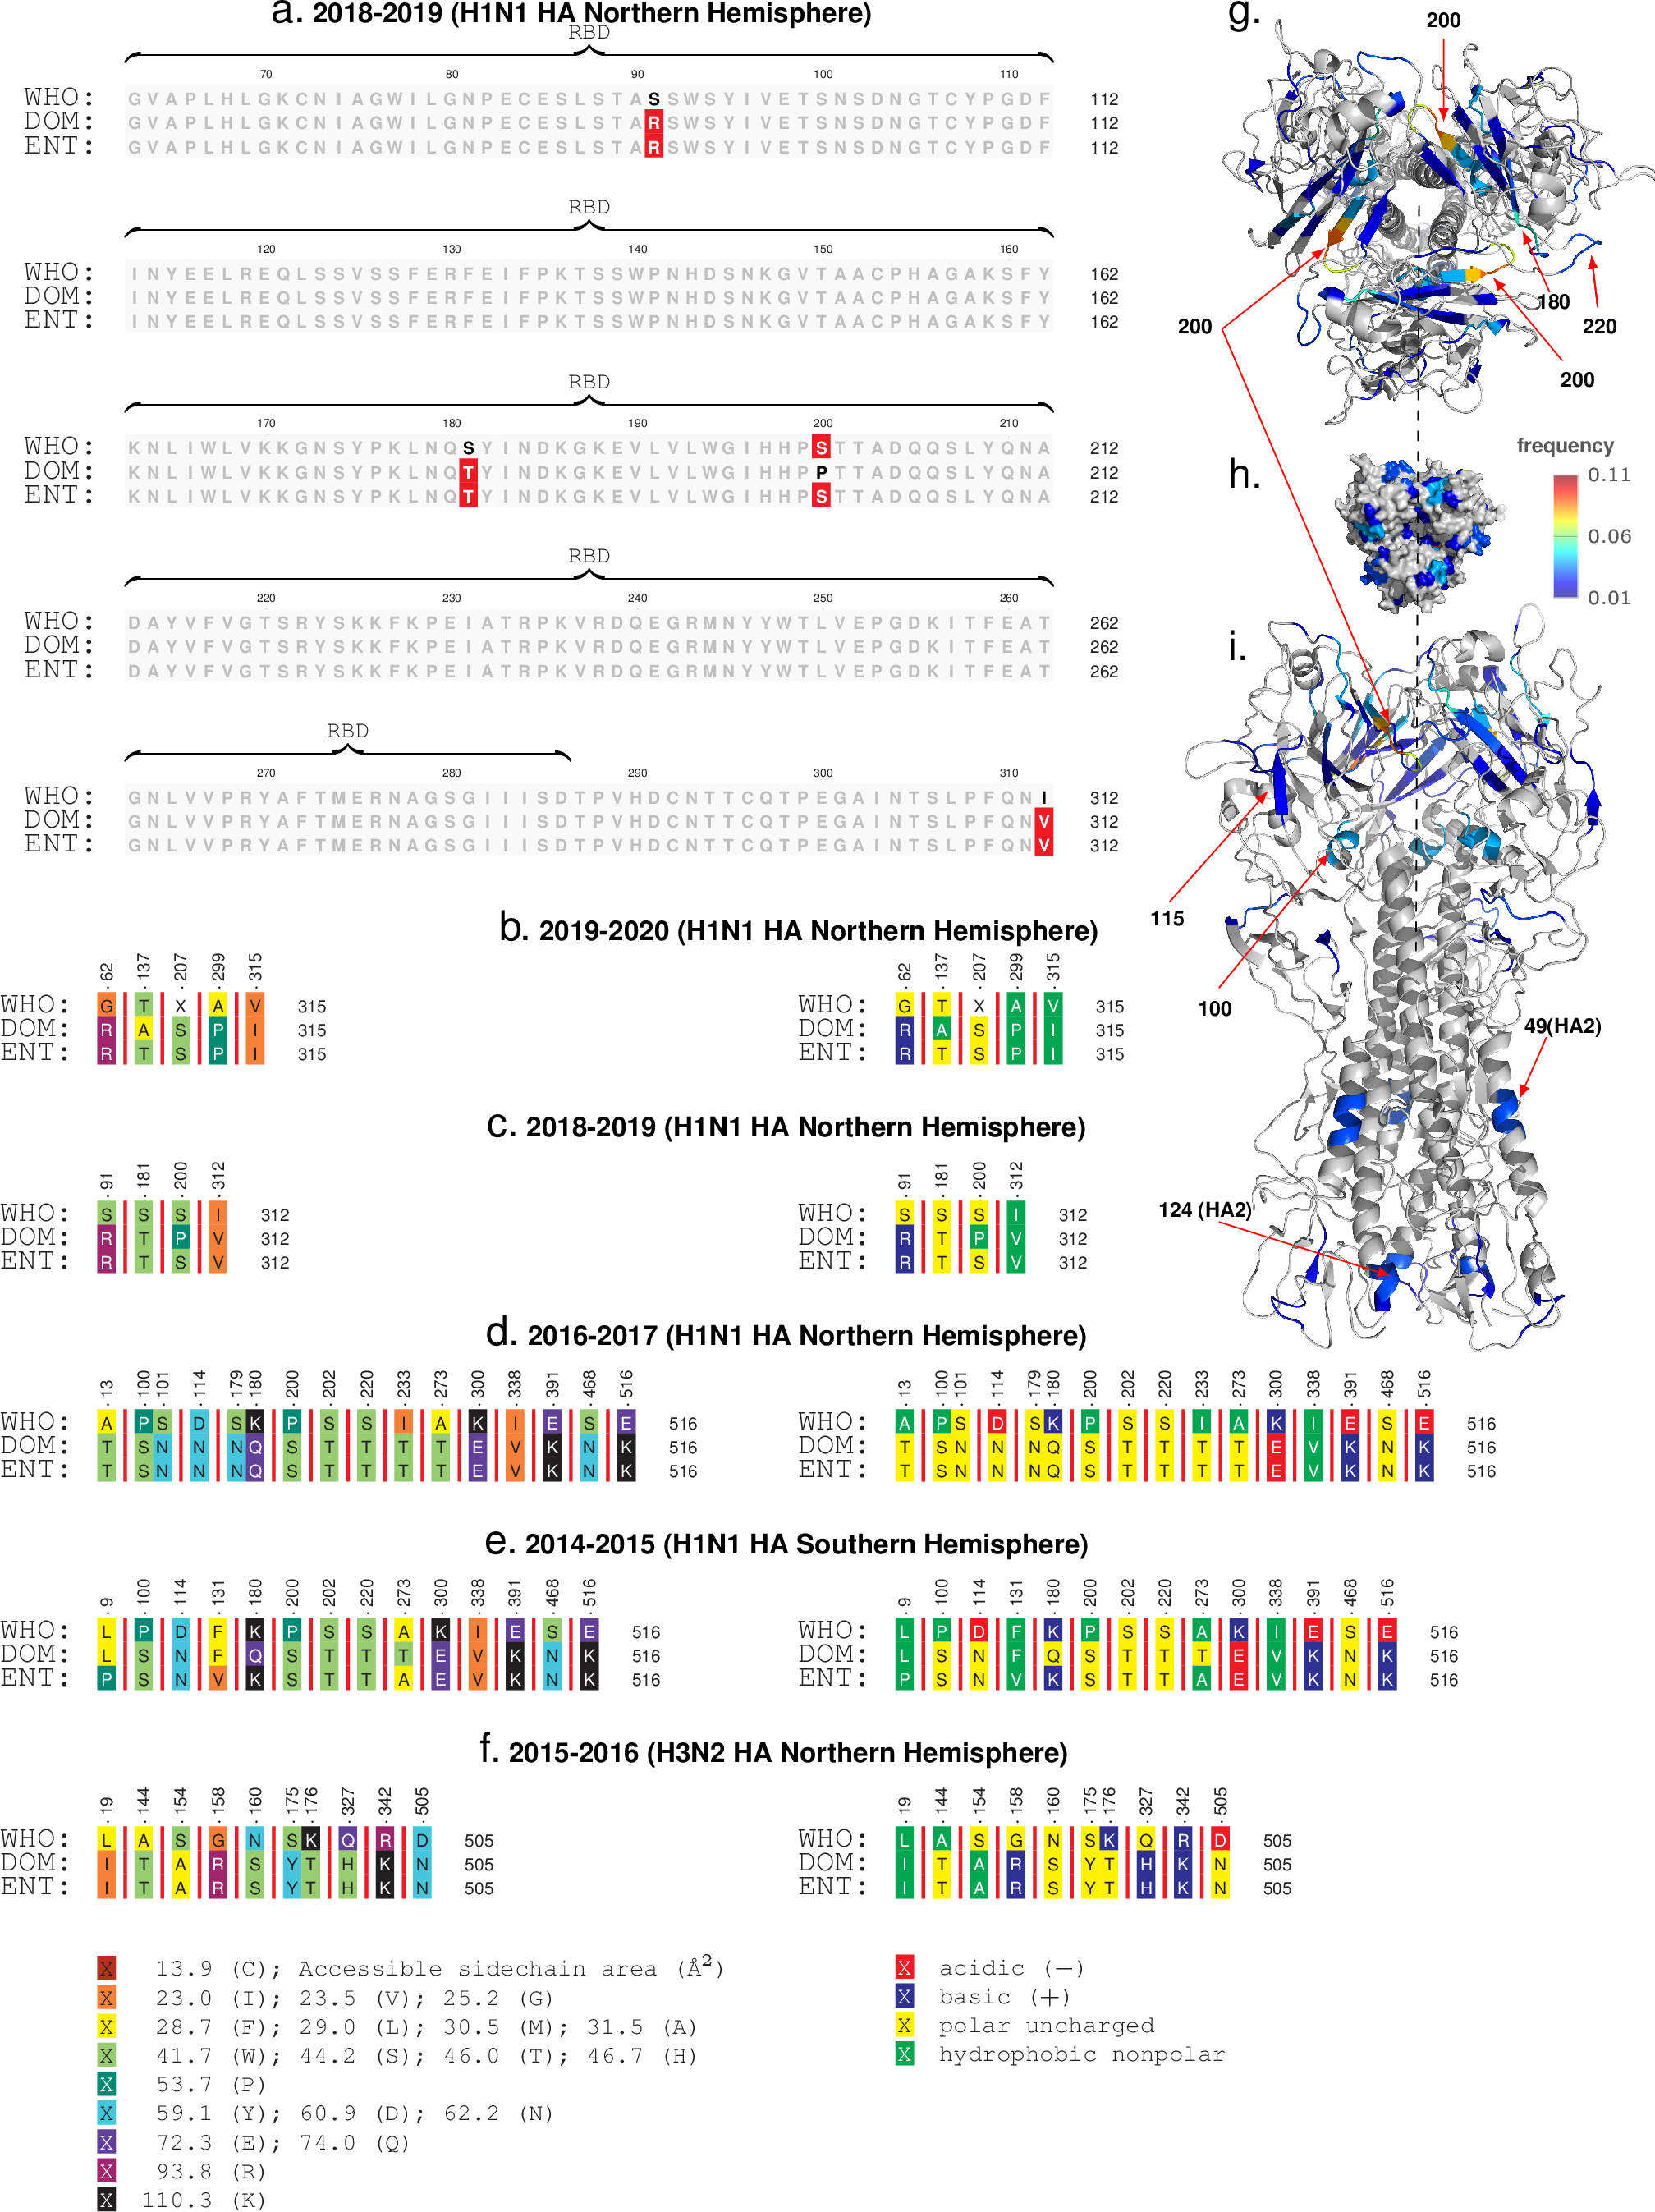
\includegraphics[width=0.87\textwidth]{Figures/External/sequence.pdf}  \vspace{-5pt}   

  \fi
\vspace{0pt}

\captionN{\textbf{Sequence comparisons.} The observed dominant strain, we note that the correct \qnet  deviations tend to be within the RBD, both for H1N1 and H3N2 for HA (panel a shows one example). Additionally, by comparing the type, side chain area, and the accessible side chain area, we note that the changes often have very different properties (panel b-f). Panels g-i show the localization of the deviations in the molecular structure of HA, where we note that the changes are most frequent in the HA1 sub-unit (the globular head), and around residues and structures that have been commonly implicated in receptor binding interactions $e.g$ the $\approx 200$ loop, the $\approx 220$ loop and the $\approx 180$-helix.}\label{figseq}
\end{figure*}
\else
\refstepcounter{figure}\label{figseq}
\fi
%#############################################
%#############################################





%#############################################
%#############################################
\def\MXCOL{black}
\def\FXCOL{Orchid3}
\def\MNCOL{SeaGreen4}
\def\FNCOL{SeaGreen4}
\def\NCOL{SeaGreen4}
\def\XCOL{Tomato}
\def\WCOL{Tomato}
\def\YCOL{DodgerBlue4}
\def\TEXTCOL{gray}
\def\AXISCOL{white}

% Bibliography
%\bibliography{qnet,BibLib1,bioshock_refs,bioshock,keck}
% \bibliographystyle{vancouver}
\bibliographystyle{naturemag}
\bibliography{allbib}

% \bibliographystyle{naturemag}

\end{document}